%%%%%%%%%%%%%%%%%%%%%%%%%%%%%%%%%%%%%%%%%%%%%%%%%%%%%%%%%%%%%%%%%%%%%%%%%%%%%%%%
\chapter{Traffic Modeling and Algorithms}\label{ch:modeling-evaluation}
%%%%%%%%%%%%%%%%%%%%%%%%%%%%%%%%%%%%%%%%%%%%%%%%%%%%%%%%%%%%%%%%%%%%%%%%%%%%%%%%


In this chapter, we are going to go into deep details on some implementations and modeling approaches mentioned in the last chapter. In the first section, we are going to discuss our methodology for modeling inter packet-times, and proof that it is a good choice. But before putting our hands on the problem, we need to precisely define what we want. We abstract our ideas in the bullets below:

\begin{itemize}    
    \item Given a set of empiral inter-packet times, we want to parametrize not only one, bua a set of "candidates" stochastic functions to describe it
    \item We want to know, analitically,  which of these candidates is the best, avoiding human analysis;
    \item We need a proof that our choosen analifical analysis is good or not to describe inter-packet times.
\end{itemize}

In the second section, we will describe and discuss the methods we used to estimate the packet-trains sizes (ON/OFF times), and to do the application classification. The calculation of the packet trains periods in our model is deterministic. The \textit{compact trace descriptor} stores the same ON and OFF times from each flow from the original traffic trace. The application classification is made by a match table of transport protocols and ports. 

\section{Inter Packet Times Modelling}

\subsection{About Inter packet time and packet trains modeling}

There are many works devoted to studying the nature of the Ethernet traffic\cite{selfsimilar-ethernet}. Classic Ethernet models used Poisson related processes to express generation of traffic. Initially, it makes sense since a Poisson process represents the probability of events occur with a known average rate, and independently of the last occurence\cite{selfsimilar-ethernet} \cite{book-poisson}. But studies made by Leland et al.\cite{selfsimilar-ethernet} showed that the Ethernet traffic has a self-similar and fractal nature. Even if they can represent the randomness of Ethernet traffic, simple Poisson processes can't express traffic "burstiness" on a long-term time scale, such as traffic "spikes" on long-range "ripples". These characteristics are an indication of the fractal and self-similar nature of the traffic, that usually we express by distributions with infinite variance, called heavy-tailed. Heavy-tail means that a stochastic distribution is not exponentially bounded\cite{sourcesonoff-paper}. Examples of heavy-tailed functions are Weibull, Pareto, Cauchy.  But heavy-tailed function may guarantee self-similarity, but not necessarily they will ensure other features like good correlation and same average packet rate.

There many consolidate works that investigate the nature of the internet traffic\cite{selfsimilar-ethernet}\cite{analysis-self-similar}\cite{stochartic-selfsimilar}\cite{selfsimilar-highvariability}\cite{multi-player-online-game-self-similarity}, and many others on the modelling of stochastic functions for specific scenarios\cite{estimation-renewal-function-ethernet-traffic}\cite{modelling-of-self-similar}\cite{empirical-interarrival-study}\cite{modeling-concurrent-heavy-tailed}\cite{optimal-scheduling-of-heavy-tailed-traffic}\cite{modelling-of-self-similar}. But not as many on model choice automation\cite{sourcesonoff-paper}.

There are plenty of works in the literature which proposes new processes and methodologies for modeling times between packets and packet trains. Fiorini \cite{modeling-concurrent-heavy-tailed} presents a heavy-tailed ON/OFF model, which tries to represent traffic generated by many sources. The model emulates a multiple source power-tail Markov-Modulated (PT-MMPP) ON/OFF process, where the ON times are power-tail distributed. They achieve analytical performance measurements using Linear Algebra Queueing Theory. Kreban and Clearwater\cite{hierarchical-dynamics-interarrival-times} presents a model for times between job submissions of multiple users over a supercomputer. They show that the Weibull probability functions can express well small and high values of inter-job submission times. They also tested exponential, lognormal and Pareto distributions. Exponential distribution couldn't represent long-range values because it fell off too fast and Pareto was too slow. Lognormal fit well small values, but was weak on larger ones. Kronewitter\cite{optimal-scheduling-of-heavy-tailed-traffic} presents a model of scheduling traffic of many heavy-tail sources. On his work, he uses many Pareto sources to represent the traffic. To estimate the shape parameter $\alpha$ they use linear regression.

In this chapter, we propose a method automatically by software. We estimate many stochastic functions through many methodologies and select the best model through the AIC computation\cite{bic-aic-comparision}. Since generating random can be costly and have a bias, depending on the seed generator, we avoid these problems since our method is analytical. We show the traffic traces we are going to use in this chapter, and in the rest of our work, and then present or selected method for parameterization and fitting choice. To test our criteria quality, we define a validation method, based on cross-validations made by simulations.

% citations
% \cite{bivariate-gamma-distribution-arrival}
% \cite{bic-aic-comparision}
% \cite{sourcesonoff-paper}
% \cite{modelling-of-self-similar}
% \cite{realtime-detection-dos}
% \cite{traffic-modelling-matlab}
% \cite{trasmission-failure}
% \cite{improvement-approaches-modeling}

\subsection{Modelling Methodology}

We start defining also define the \textit{pcaps} datasets we are going to use in the rest of this text. We will use for datasets, and for reproduction purposes, three are publicly available. 
The first is a lightweight Skype capture, found in  Wireshark wiki\footnote{https://wiki.wireshark.org/}, and can be found at \href{https://wiki.wireshark.org/SampleCaptures}{https://wiki.wireshark.org/SampleCaptures}. The file name is \texttt{SkypeIRC.cap}, and we call it \textit{skype-pcap}.

The second is a CAIDA\footnote{http://www.caida.org/home/}{http://www.caida.org/home/} capture, and can be found at  \href{https://data.caida.org/datasets/passive-2016/equinix-chicago/20160121-130000.UTC}{https://data.caida.org/datasets/passive-2016/equinix-chicago/20160121-130000.UTC}. Access to this file need login, so you will have to create an account and wait for approval first. The pcap's file name is \texttt{equinix-chicago.dirB.20160121-135641.UTC.anon.pcap.gz}. We call it \textit{wan-pcap}.

The third we capture in our laboratory LAN, through a period of 24 hours. It was captured firewall gateway between our local and external network. Along with other tests, We intend to verify diurnal behavior on it. That means a high demand of packets during the day and a small in the night. We call it \textit{lan-firewall-diurnal-pcap}.

%2nd-review
The fourth is a capture of a busy private network access point to the Internet, available online on TCPreplay website \footnote{ \href{http://tcpreplay.appneta.com/wiki/captures.html}{http://tcpreplay.appneta.com/wiki/captures.html}}, called \texttt{bigFlows.pcap}. We will refer to it \textit{lan-gateway-pcap}.


%In this chapter we will evaluate our proposed method for data modeling of inter-packet times.  We will present curves obtained by our prototype (implemented in Gnu Octave\footnote{\href{https://www.gnu.org/software/octave/}{https://www.gnu.org/software/octave/}}) that shows in detail how each step works. After explaining this process, we will present an evaluation method of our results, analyzing to analyze its quality. After this, we give some details of how we convert code from Octave to C++ and its benefits on time execution. All code used in this section is available on our GitHub page.%, on the directory \texttt{Prototypes}. 


%Along with these datasets, we will use two subpcaps from the originals. The first, \textit{skype-flowburst-pcap}, is a burst of a single HTTP flow from \textit{skype-pcap}. It can be obtained from Wireshark using the filter \texttt{(ip.src\_host==172.16.133.25) \&\& (ip.dst\_host==74.125.170.42) \&\& (tcp.dstport==80) \&\& (tcp.srcport==63378) \&\& (frame.time\_relative>30.0) \&\&( frame.time\_relative<50.0)}. The second, \textit{caida1s-pcap} is a trace with the first second from \texttt{wan-pcap}.


%2nd-review
We summarize our process of modeling inter-packet times at the figure~\ref{fig:model-parameterization}. We collect a set of inter-packet times from an actual traffic capture. Then, we estimate a set of parameters for stochastic functions, using different methodologies. Then, from these parametrized models, we determine which best represent our data set, using the measure of quality AIC (Akaike information criterion). We also calculate another ratio of quality called BIC (Bayesian information criterion), for comparison of results. In this chapter, we present our results obtained on our prototype implemented in Octave\footnote{ \href{https://www.gnu.org/software/octave/}{https://www.gnu.org/software/octave/}}. 

Currently, we are modeling:

\begin{itemize}
    \item Weibull distribution, using linear regression, through the Gradient descendant algorithm;
    \item Normal distribution, using direct calculation of the average and the standard deviation of the inter-packet times from the dataset;
    \item Exponential distribution, using linear regression, through the Gradient descendant algorithm. We refer to this distribution as Exponential(LR);
    \item Exponential distribution, using a rate estimation form the dataset. We refer to this distribution as Exponential(Me);
    \item Pareto distribution, using linear regression, through the Gradient descendant algorithm. We refer to this distribution as Pareto(LR);
    \item Pareto distribution, using the maximum likelihood method. We refer to this distribution as Pareto(MLH);
    \item Cauchy distribution, using linear regression, through the Gradient descendant algorithm;
\end{itemize}

%\textcolor{red}{TODO: Explciar quais dados são armazenados na base de dados e por que. Explicar como os dados são classificados, e modelados, e os parametros gerados. Citar métodos utilizado para parametrização, como calculo da média, maximmum likelihood e regressão linear. Apredentar o diagrama da ultima apresentação. Apresentar as equações utilizadas. Com esses dados bem como os plots dos dados linearizados, da corvergencia do custo e o fitting da CDF. Apresentar uma tabela com o valor do BIC e AIC para cada fitting. (Vai ficar muito grande a sessão)}

% In probability theory and statistics, the exponential distribution (a.k.a. negative exponential distribution) is the probability distribution that describes the time between events in a Poisson process, i.e., a process in which events occur continuously and independently at a constant average rate. It is a particular case of the gamma distribution. It is the continuous analog of the geometric distribution, and it has the crucial property of being memoryless. In addition to being used for the analysis of Poisson processes, it is found in various other contexts.

Now we will give a brief explanation our three procedures: Linear Regression (with the  Gradient descendant algorithm), direct estimation, and maximum likelihood. Some observations must be made. Since the time samples resolution used were of $10^{-6}$s, all values equal to zero were set to  $5\cdot10^{-8}$s, to avoid division by zero. To avoid divergence in tangent operation used in the linearization of the Cauchy function, we floor-limited and upper-limited the inter-packet CDF  values by  $10^{-6}$ and $0.999999$, respectively. We implemented this prototype using Octave. We upload the code on GitHub, for reproduction purposes\footnote{\href{https://github.com/AndersonPaschoalon/ProjetoMestrado/tree/master/Tests/PrototypeDataProcessor}{https://github.com/AndersonPaschoalon/ProjetoMestrado/tree/master/Tests/PrototypeDataProcessor}}

%We go deep into details explaining the methods on the appendix ~\ref{ap:revision-probability}, and present the mathematical demonstrations on appendix~\ref{ap:revision-probability}. 

\subsubsection{Linear regression (Gradient descendant)}

Linear regression is a method for estimating the best linear curve in the format:

\begin{equation}
y = ax + b
\end{equation}

to fit a given data set. We can use linear regression to estimate parameters of a non-linear curve expressing it on a linear format. For example, the Weibull CDF for $t > 0$ is:

\begin{equation}
F(t|\alpha, \beta) = F(t) = 1 - e^{-(t/\beta)^{\alpha}}
\end{equation}

Manipuling the equation:
\begin{equation}
\alpha\ln{(t)} - \alpha\ln{(\beta)} = \ln{(-\ln{(1 - F(t))})}
\end{equation}


If we call $x = \ln{(t)}$ and $y = \ln{(-\ln{(1 - F(t))})}$, we found a linear equation, where $a = \alpha$ and $b = -\alpha\ln{(\beta)}$. Having in hands a estimation of the empirical CDF of our data samples, we apply the $x$ and $y$ definitions to linearize the data. 

Using the gradient descendant, we find an estimation of the linear coefficients $\hat{a}$ and $\hat{b}$. Using the inverse function of linear factors, we see the Weibull estimated parameters $\hat{\alpha}$ and $\hat{\beta}$.

\begin{equation}
\alpha = a
\end{equation}

\begin{equation}
\beta = e^{-(b/a)}
\end{equation}

The gradient descendent consists in minimizing a cost function $J(\theta)$. We explain this procedure in the appendix ~\ref{ap:revision-probability}. In the figure~\ref{fig:linearization} we present as examples, the linearized data for the inter arrivals from the \textit{skype-pcap}, and in the figure ~\ref{fig:cost} the cost convergence. In the appendix ~\ref{ap:aditional-plots}, a complete set of these figures is presented.

Applying the inverse equations of the linear coefficients ($\hat{\alpha} = \hat{a}$ and $\hat{\beta} = e^{-(\hat{b}/\hat{a})}$) \footnote{The hat symbol ( $ \widehat{} $ ) for the estimated parameters}, we are able to estimate the Weibull distribution parameters. We can summarize this procedure, in these steps:
\begin{enumerate}
\item Linearize the stochastic CDF function F(t).
\item Apply the linearized $y = y(F(t))$ and  $x = x(t)$ on the empirical CDF and times datasets, respectively. 
\item Use Gradient Descendant algorithm to find linear coefficients $a$ and $b$.
\item Apply the inverse equation of the linear coefficients, to determine the stochastic function parameters.
\end{enumerate}

In the parameters estimation (step 4), there is an exception, since the Pareto scale ($t_{m}$) is defined by the minimum time. In the table~\ref{tab:linearization-sumary} we present a summary of the used equations in the procedure. In this notation, the subscript $i$ means that it must be applied to every value measured empirically. The hat( $\widehat{}$ ) indicates an estimated value for a parameter. 

\begin{table}[h!]
    \centering
    \caption{Linearized functions, and parameters estimators, used by the linear regression}
    \label{tab:linearization-sumary}
    \begin{tabular}{llllll}
        \hline
        Function    & Linearized $x$     & Linearized $y$                    & \multicolumn{2}{l}{Parameters Estimator}                               &  \\
        \hline
        Cauchy      & $x_i = t_i$        & $y_i = \tan{(\pi(F(t_i) - 1/2))}$ & $\hat{\gamma} = \frac{1}{\hat{a}}$ & $\hat{t_0} = - \frac{\hat{b}}{\hat{a}}$                      &  \\
        Exponential & $x_i = t_i$        & $y_i = \ln{(1 - F(t_i))})$        & \multicolumn{2}{l}{$\hat{\lambda} = -\hat{a}$}                                              &  \\
        Pareto      & $x_i = \ln{(t_i)}$ & $y_i = \ln{(1 - F(t_i))}$         & $\hat{\alpha} = -\hat{a} $         & $\hat{x_{m}} = \min_{i = 0, ..., m}\{x_{i}\}$ &  \\
        Weibull     & $x = \ln{(t)}$     & $y = \ln{(-\ln{(1 - F(t))})}$     & $\hat{\alpha} = \hat{a}$                 & $\hat{\beta} = e^{-(\hat{b}/\hat{a})}$                                   & \\
        \hline
    \end{tabular}
\end{table}



\begin{figure}[ht!]
\centering
\subfloat[Linearized interarrival data]{
  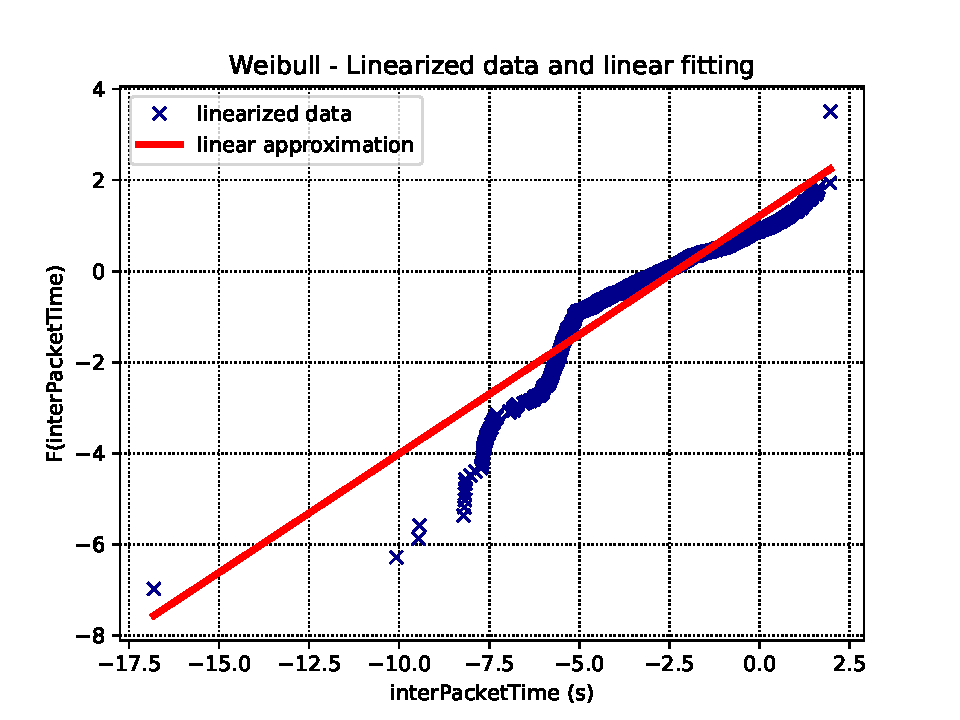
\includegraphics[height=50mm]{figures/ch4/Skype_Weibull_-_Linearized_data_and_linear_fitting}
  \label{fig:linearization}
}
%\hspace{0mm}
\subfloat[Cost function of the linear regression]{
  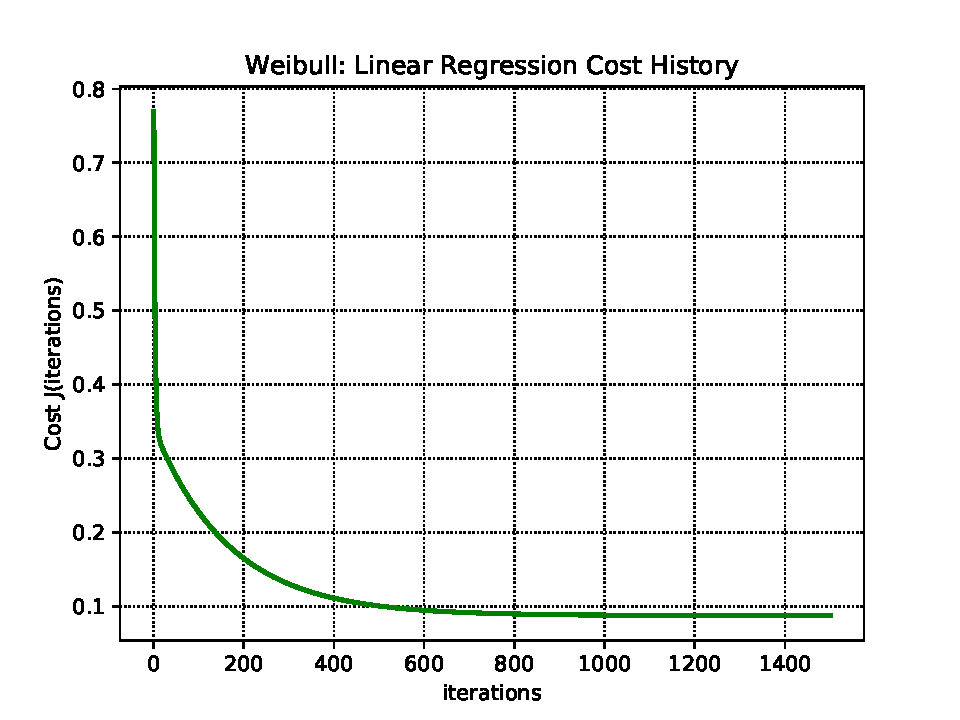
\includegraphics[height=50mm]{figures/ch4/Skype_Weibull_-_Cost_J(iterations)_convergence}
  \label{fig:cost}
}
\label{fig:linearization-cost}
\caption{Linearized data and cost function of weibull linear regression}
\end{figure}



\subsubsection{Direct Estimation}

%2nd-review
The expected value $E(X)$ and variance $Var(X)$ of a random variable $X$ of some distributions are closely related to its parameters. Since the average $\bar{\mu}$ and its standard deviation $\bar{\sigma}$ are in general good approximations for the expected value and variance, we use them to estimate parameters.

%2nd-review
Following the notation presented at table~\ref{tab:distributions-equations}, we have for the normal distribution:
\begin{equation}
(\hat{\mu}, \hat{\sigma} = (\bar{\mu}, \bar{\sigma})
\end{equation}

%2nd-review
For the exponential distribution $E(X) = \frac{1}{\lambda}$, therefore we have:
\begin{equation}
\hat{\lambda} = \frac{1}{\hat{\mu}}
\end{equation} 

\subsubsection{Maximum Likelihood}


The maximum likelihood estimation, is a method for estimation of parameters, winch maximizes the likelihood function. We explain in details this subject in the Appendix A. Using this method for the Pareto distribution, it is possible to derive the following equations the its parameters:

\begin{equation}
\hat{x_{m}} = \min_{i = 0, ..., m}\{x_{i}\}
\end{equation} 

\begin{equation}
\hat{\alpha} = \frac{n}{ \sum_{i = 0}^{m}(\ln{(x_{i}) - \ln(\hat{x_{m}})})  }
\end{equation} 

where $m$ is the sample size.


\subsection{Modelling Method Validation}

To see if our criterion of parameter selection is can find which is the best model, we define a validation methodology. 
We generate a vector with the same size form the original, with randomly generated data through our model estimation. Then we compare it with the original sample, trough four different metrics, all with a confidence interval of 95\%:

\begin{itemize}
\item Correlation between the sample data and the estimated model (Pearson's product-moment coefficient);
\item Hurst exponent;
\item Mean inter-packet time;
\item Standard deviation of inter-packet times.
\end{itemize}

The Pearson's product-moment coefficient, or simply correlation coefficient,  is an expression of the dependence or association between two datasets. Its value goes from -1 to +1. +1 means a perfect direct linear correlation. -1 indicates perfect inverse linear correlation. 0 means no linear correlation. So, as close the result reaches 1, more similar are the inter-packet times to the original values. To estimate it, we use the Octave's function \texttt{corr()}.

As explained before in the chapter~\ref{ch:literature-review}, the Hurst exponent is meter self-similarity and indicates the fractal level of the inter-packet times. As close the result is from the original, more similar is the fractal level of the estimated samples from the original. To determine this value, we use the function \texttt{hurst()} from Octave, which uses rescaled range method.
Finally we measure the mean and the standard deviation (as a measure of the dispersion), using the Octave's functions \texttt{mean()} and \texttt{std()}. We also present some \textit{QQplots}, to visually compare the random-generated data and the original dataset. 

As close the correlation, Hurst exponent, average and the standard deviation is from the original dataset, the better is model fitting. Also, analyzing the average, we can see if a particular modeling procedure tends to be more penalized for the values close, or far from zero. This means that if the average inter-packet time tends to be smaller or higher compared to the original. 

With these results in hands, we can see if AIC and BIC are reasonable criteria for model selection for inter-packet times. To quantitatively check it, we define a cost function based on the correlation, Hurst exponent and mean. We exclude the standard deviation, because the Hurst exponent being a meter of the fractal level, also capture information about the desired dispersion of the data. So, for comparing all these results, we defined a cost function $J$, based on the randomly generated data values.

Being $Cr$ the vector of correlations ordered from greater to the smaller, let $Me$ and $Hr$ defined by the absolute difference between average and hurt exponent of the estimated values and the original dataset. Both are ordered from the smaller to the greatest values. Letting $\phi(V, M)$ be an operator which gives the position of a model $M$ in a vector $V$, we define the cost function $J$ as:


\begin{equation}
J(M) = \phi(Cr, M) + \phi(Me, M) + \phi(Hr, M)
\end{equation}

The smaller is the cost $J$, the best is the model. Then we compare the results achieved by AIC and BIC, and $J$.

\subsection{Modelling Results}

%%%%%%%%%%%%%%%%%%%%%%%
% Logscale Skype
%%%%%%%%%%%%%%%%%%%%%%%
\begin{figure}[ht!]
\centering
\subfloat[Chauchy]{
  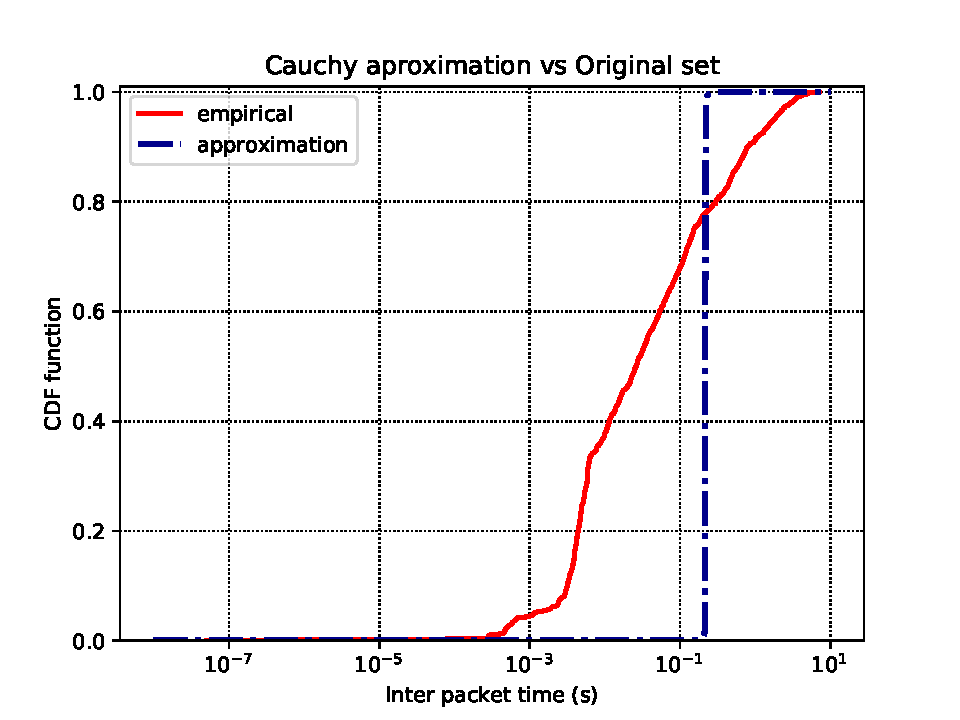
\includegraphics[width=62mm]{figures/ch4/Skype_Log_-_Cauchy_aproximation_vs_Original_set}
}
\subfloat[Exponential(LR)]{
  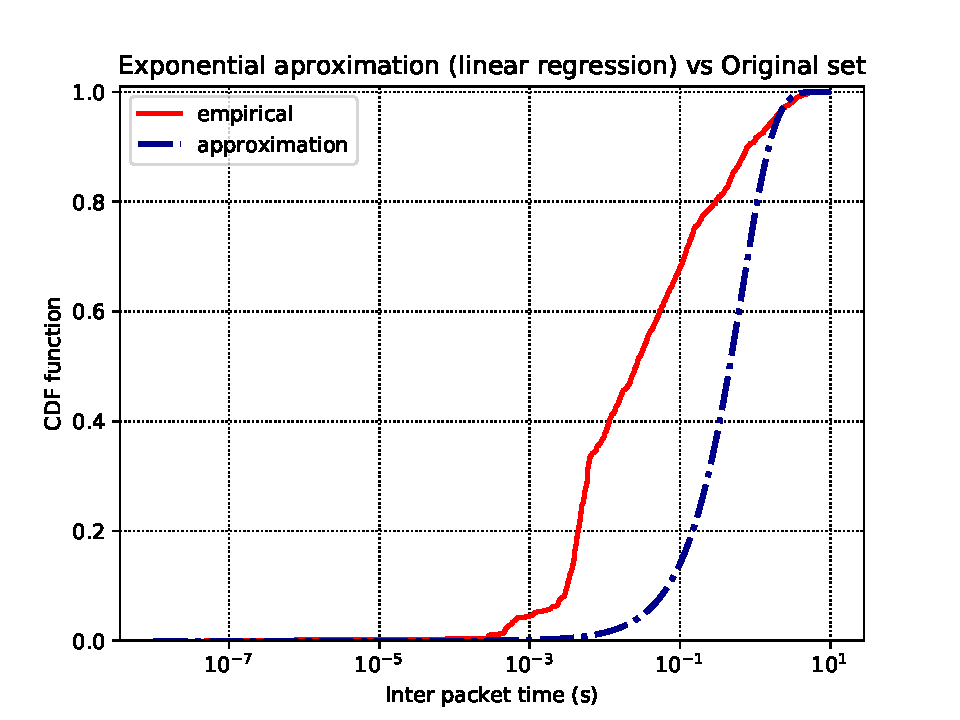
\includegraphics[width=62mm]{figures/ch4/Skype_Log_-_Exponential_aproximation_(linear_regression)_vs_Original_set}
}
\hspace{0mm}
\subfloat[Exponential(Me)]{
  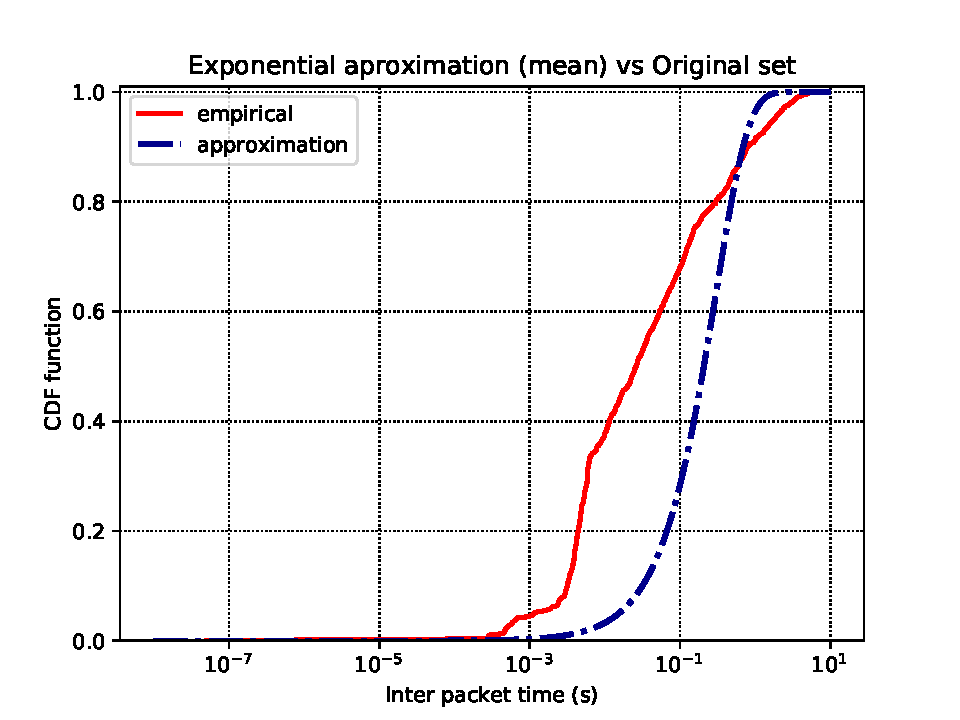
\includegraphics[width=62mm]{figures/ch4/Skype_Log_-_Exponential_aproximation_(mean)_vs_Original_set}
}
\subfloat[Normal]{
  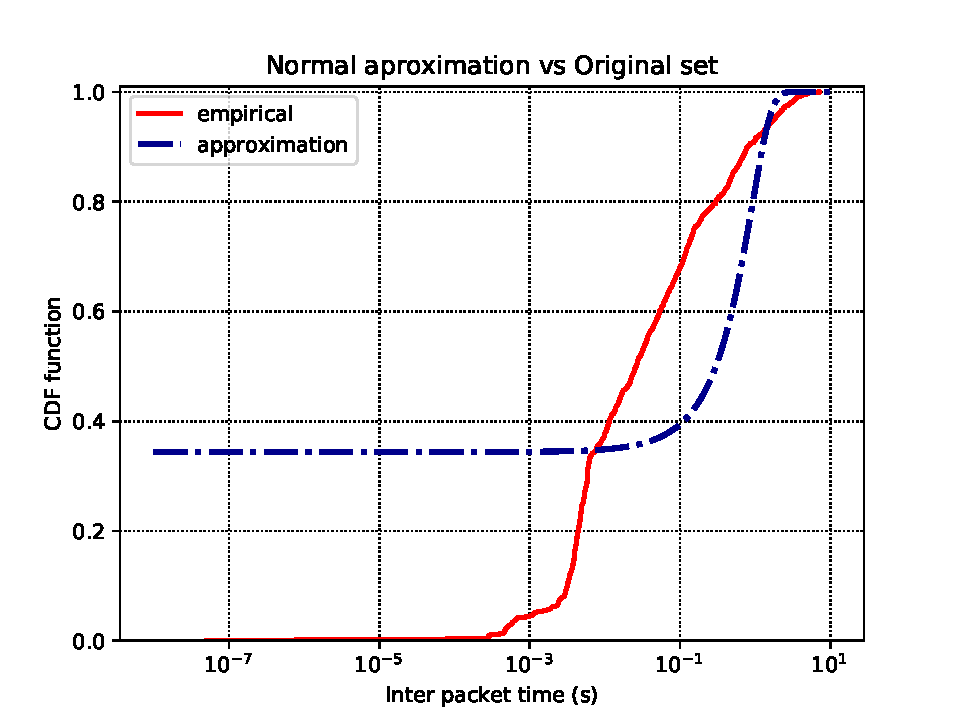
\includegraphics[width=62mm]{figures/ch4/Skype_Log_-_Normal_aproximation_vs_Original_set}
}
\hspace{0mm}
\subfloat[Pareto(LR)]{
  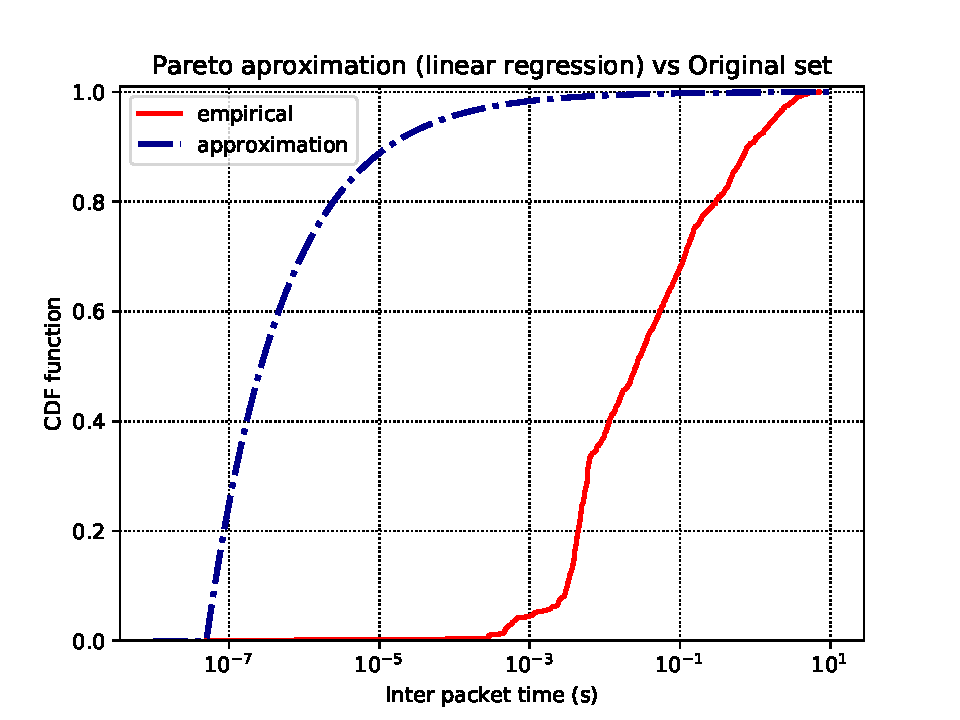
\includegraphics[width=62mm]{figures/ch4/Skype_Log_-_Pareto_aproximation_(linear_regression)_vs_Original_set}
}
\subfloat[Pareto(MLH)]{
  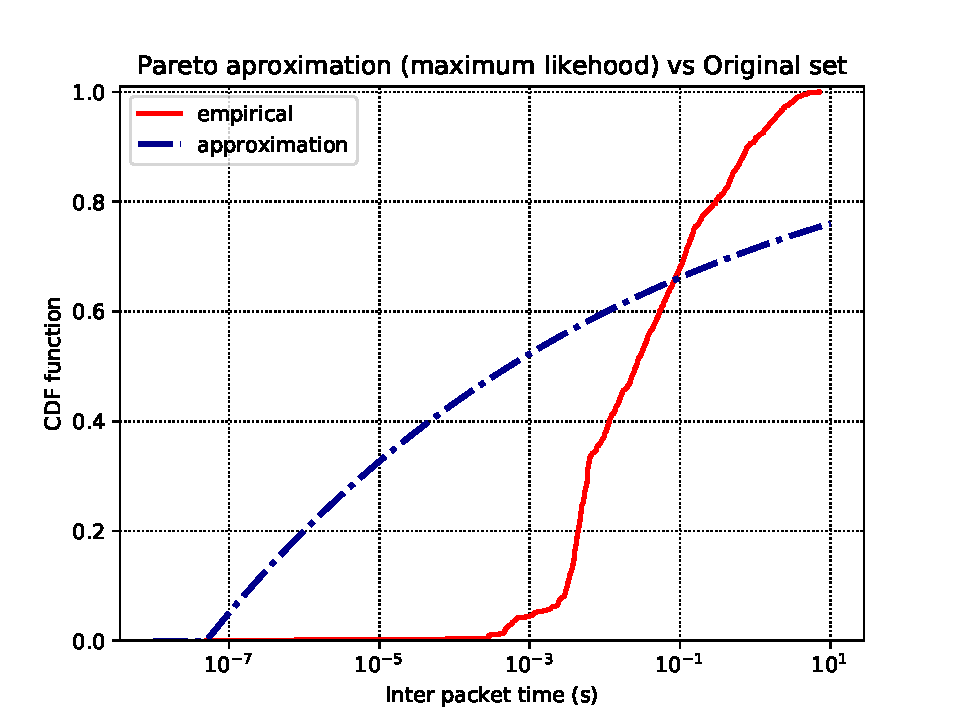
\includegraphics[width=62mm]{figures/ch4/Skype_Log_-_Pareto_aproximation_(maximum_likehood)_vs_Original_set}
}
\hspace{0mm}
\subfloat[Weibull]{
  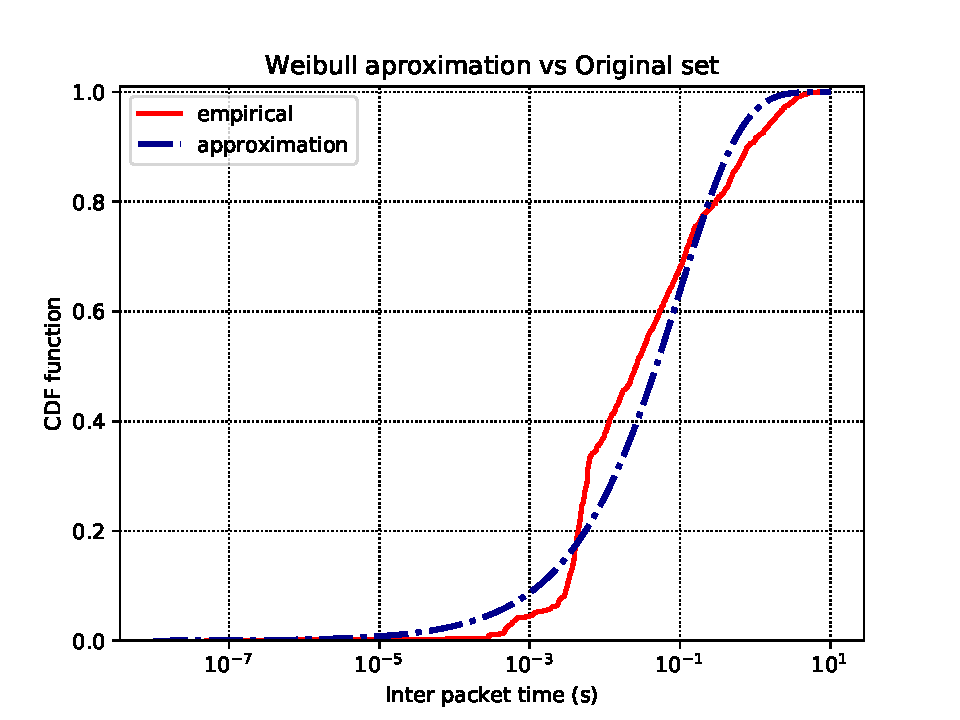
\includegraphics[width=62mm]{figures/ch4/Skype_Log_-_Weibull_aproximation_vs_Original_set}
}
\label{fig:aproximation-original-cdf}
\caption{CDF functions for the approximations of \textit{skype-pcap} inter  packet times, of many stochastic functions.}
\end{figure}

%%%%%%%%%%%%%%%%%%%%%%%
% QQplots Skype
%%%%%%%%%%%%%%%%%%%%%%%
\begin{figure}[ht!]
    \centering
    \label{fig:qq-skype}
    \subfloat[Chauchy]{
        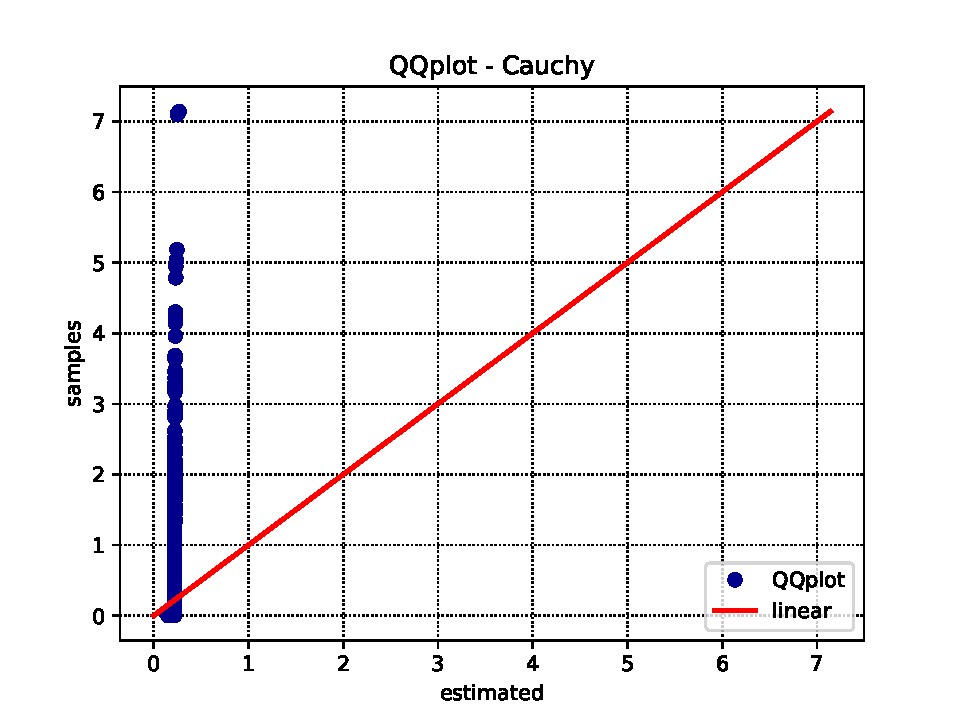
\includegraphics[width=62mm]{figures/ch4/Skype_QQplot_-_Cauchy}
    }
    \subfloat[Exponential(LR)]{
        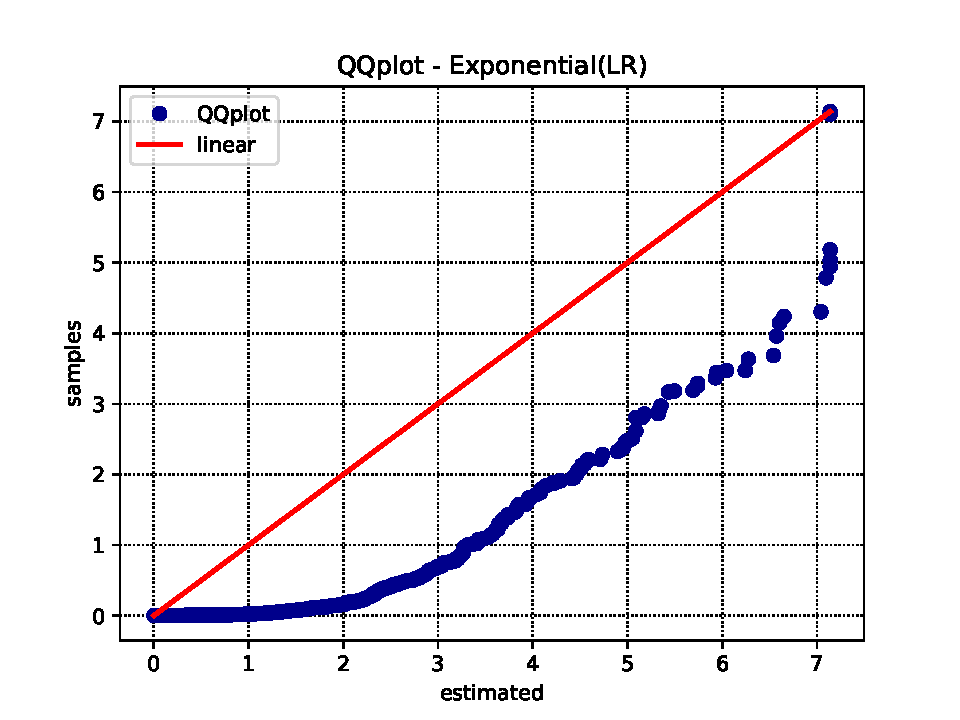
\includegraphics[width=62mm]{figures/ch4/Skype_QQplot_-_Exponential(LR)}
    }
    \hspace{0mm}
    \subfloat[Exponential(Me)]{
        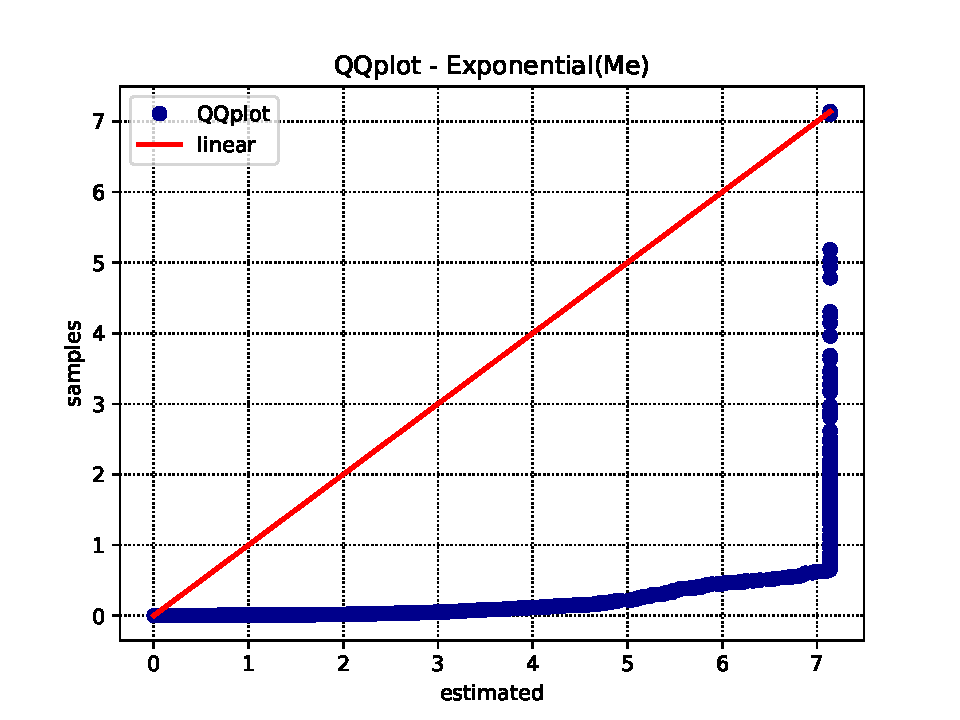
\includegraphics[width=62mm]{figures/ch4/Skype_QQplot_-_Exponential(Me)}
    }
    \subfloat[Normal]{
        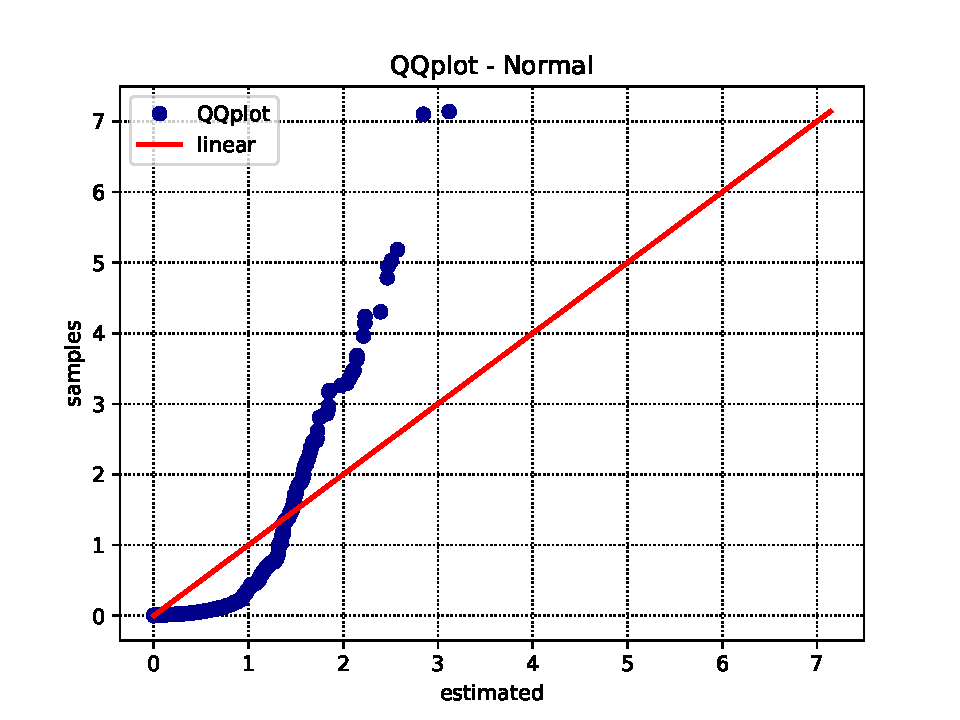
\includegraphics[width=62mm]{figures/ch4/Skype_QQplot_-_Normal}
    }
    \hspace{0mm}
    \subfloat[Pareto(LR)]{
        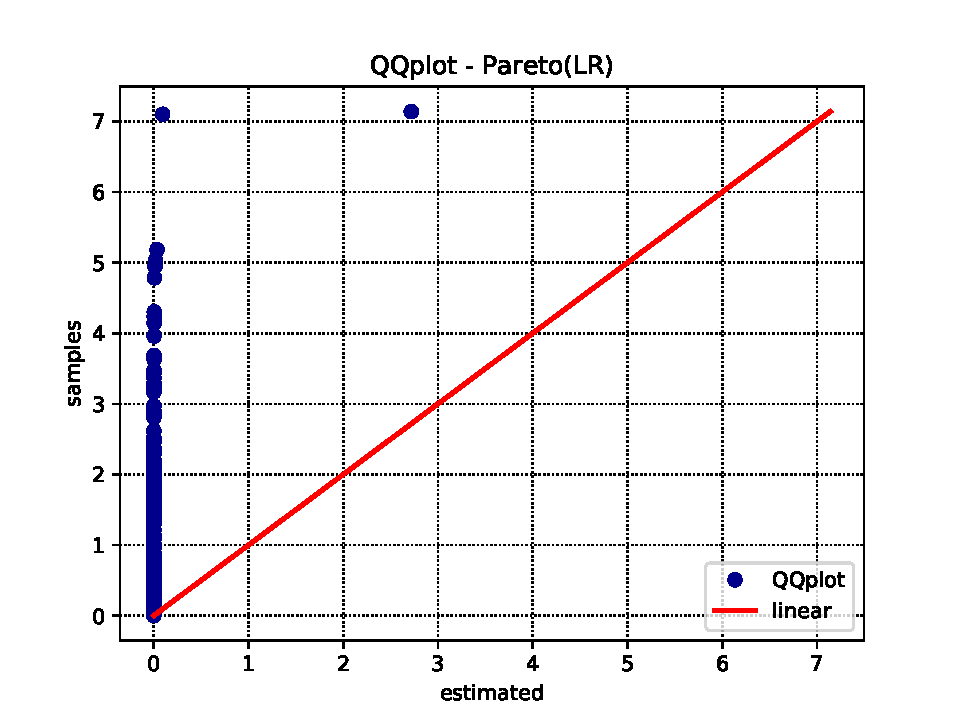
\includegraphics[width=62mm]{figures/ch4/Skype_QQplot_-_Pareto(LR)}
    }
    \subfloat[Pareto(MLH)]{
        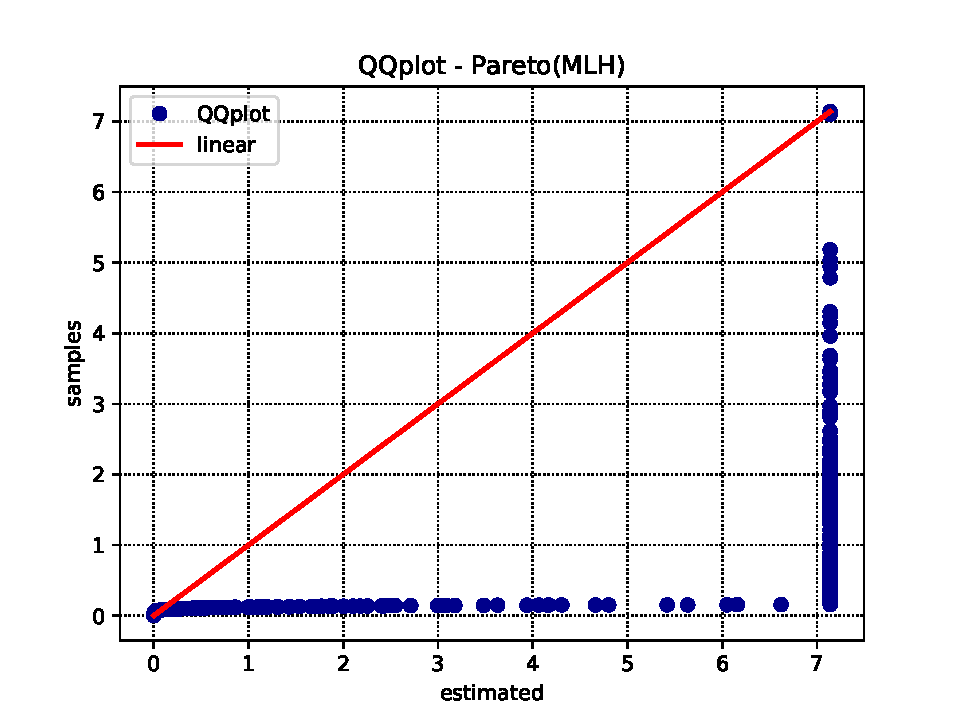
\includegraphics[width=62mm]{figures/ch4/Skype_QQplot_-_Pareto(MLH)}
    }
    \hspace{0mm}
    \subfloat[Weibull]{
        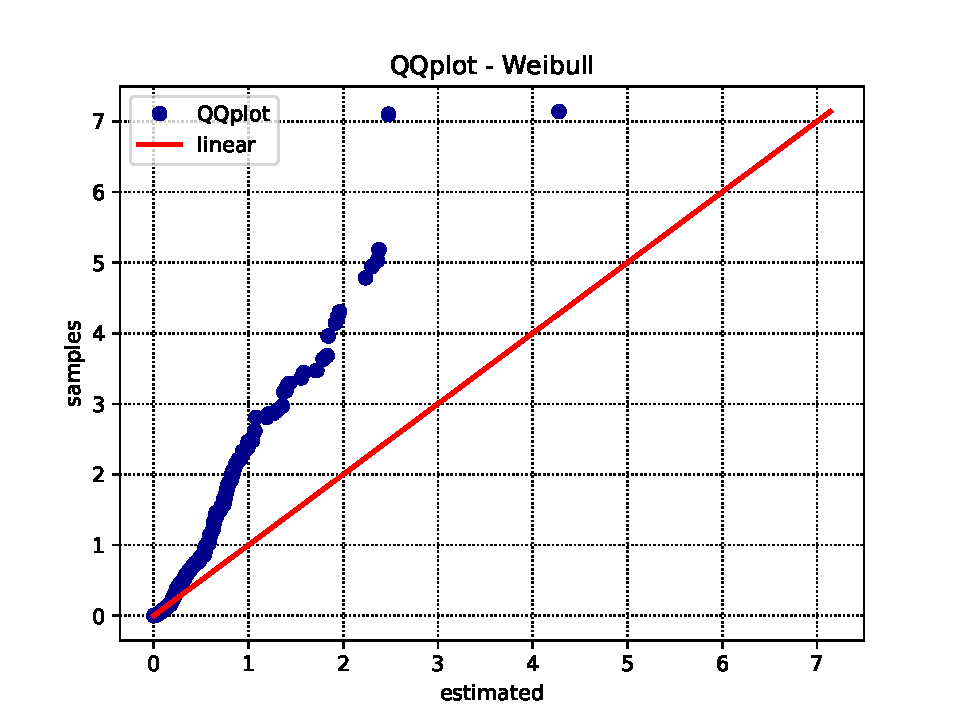
\includegraphics[width=62mm]{figures/ch4/Skype_QQplot_-_Weibull}
    }
    \caption{CDF functions for the approximations of \textit{skype-pcap} inter packet times, of many stochastic functions.}
\end{figure}

%%%%%%%%%%%%%%%%%%%%%%%
% Simulation table
%%%%%%%%%%%%%%%%%%%%%%%
\begin{sidewaystable}[!hp]
	\centering
    \caption{3 Results of the octave prototype, include BIC and AIC values, para estimated parameters for our pcap traces}
        \begin{threeparttable}[t]
        \begin{tabular}{lcccccccccc}
            \hline
            & \multicolumn{10}{c}{Trace} \\ \cline{2-11} 
            Function        & Order & AIC  & BIC  & \multicolumn{2}{c}{Parameters}  
            & Order & AIC & BIC  & \multicolumn{2}{c}{Parameters} \\ \hline 
            
            & \multicolumn{5}{c}{skype-pcap}  & \multicolumn{5}{c}{lan-diurnal-firewall-pcap}   \\ \hline 
            Cauchy          &    7 & $1.35e4$    & $2.19e4$    & $\gamma:2.75e-4$ & $x_0:2.19e-1$    
            &    5 & $-2.85e7$   & $-2.85e7$   & $\gamma:9.63e-3$ & $x_0:-3.61e-3$    \\
            Exponential(LR) &    3 & $9.69e1$   & $1.02e2$   & \multicolumn{2}{c}{$\lambda:1.51$}   
            &    6 & $1.79e6$    & $1.79e6$    & \multicolumn{2}{c}{$\lambda:8.51e-1$}    \\
            Exponential(Me) &    2 & $-4.26e2$   & $-4.28e3$   & \multicolumn{2}{c}{$\lambda:3.32$}   
            &    4 & $-3.12e7$   & $-3.12e7$   & \multicolumn{2}{c}{$ \lambda:58.78$} \\
            Normal          &    5 & $2.42e3$    & $3.31e3$    & $\mu:3.01e-1 $    & $\sigma:7.49e-1$ 
            &    7 & $Inf \tnote{1}$       & $Inf \tnote{a}$       & $\mu:1.70e-2$     & $\sigma:8.56e-2$ \\
            Pareto(LR)      &    6 & $6.4e3$   & $-8.27e3$   & $\alpha:4.14e-1$ & $x_m:5e-8$    
            &    3 & $-4.60e7$   & $-4.60e7$   & $\alpha:2.55e-1$ & $ x_m:5e-8$    \\
            Pareto(MLH)     &    4 & $3.62e2$   & $3.72e2$   & $\alpha:7.47e-2$ & $x_m:5e-8$    
            &    2 & $-5.03e7$   & $-5.03e7$   & $\alpha:1.15e-1$ & $ x_m:5e-8$    \\
            Weibull         &    1 & $-2.29e3$   & $-2.28e3$  & $\alpha:5.22e-1$ & $\beta:9.77e-2$  
            &    1 & $-5.60e7$   & $-5.60e7$   & $\alpha:3.34e-1$ & $\beta:1.83e-3$  \\ \hline    
            & \multicolumn{5}{c}{lan-gateway-pcap} & \multicolumn{5}{c}{wan-pcap}  \\ \hline
            Cauchy          &    6 & $7.14e6$    & $7.14e6$   & $\gamma:1.94e0$ &$x_0:-7.25$    
            &    7 & $5.99e7$    & $5.99e7$   & $ \gamma:8.28e2$ &$x_0:-4.52e3$    \\
            Exponential(LR) &    7 & $7.33e6$    & $7.33e6$   & \multicolumn{2}{c}{$\lambda:1.489e-1$}   
            &    6 & $5.68e7$    & $ 5.68e7$  & \multicolumn{2}{c}{$\lambda:2.2e-5$}   \\
            Exponential(Me) &    2 & $-1.09e7$   & $-1.09e7$  & \multicolumn{2}{c}{$\lambda:2.64e3$}   
            &    1 & $-6.58e7$   & $-6.58e7$  & \multicolumn{2}{c}{$\lambda:6.58e5$} \\
            Normal          &    5 & $-9.35e6$   & $-9.35e6$  & $\mu:3.79e-4$   &$\sigma:6.60e-4$ 
            &    2 & $-6.39e7$   & $-6.39e7$  & $\mu:2e-6$     & $\sigma:1e-6$ \\
            Pareto(LR)      &    4 & $-1.02e7$   & $-1.02e7$  & $\alpha:1.489e-1 $ & $x_m:5e-8 $    
            &    4 & $-5.31e7$   & $-5.31e7$  & $\alpha:4e-14\tnote{b}$ & $x_m:5e-8 $    \\
            Pareto(MLH)     &    3 & $-1.03e7$   & $-1.03e7$  & $\alpha:1.362e-1$ & $x_m:5e-8 $    
            &    5 & $-6.25e7$   & $-6.25e7$  & $\alpha:3.39e-1$ & $x_m:5e-8 $    \\
            Weibull         &    1 & $-1.10e7$   & $-1.10e7$  & $\alpha:2.81e-1$ & $\beta:5.54e-4$  
            &    3 & $-5.46e7$   & $-5.46e7$  & $\alpha:7.64e-2$ & $\beta:1e-6$  \\ \hline
        \end{tabular}
            \begin{tablenotes}
            \item[1] The computation of the likelihood function has exceeded the computational precision used, so it was the highest AIC and BIC  for this trace.
            \item[2] The linear regression did not converge to a valid value, so we used a small value("infinitesimal") instead to perform the computations.
            \end{tablenotes}
        \end{threeparttable}
    \label{tab:prototype-results}
\end{sidewaystable}

%%%%%%%%%%%%%%%%%%%%%%%
% AIC BIC  diff
%%%%%%%%%%%%%%%%%%%%%%%
\begin{table}[]
\centering
\caption{Relative difference between $AIC$ and $BIC$.}
\begin{tabular}{ccccc}
\hline
& skype-pcap  & \begin{tabular}[c]{@{}c@{}}lan-gateway-\\ pcap\end{tabular} & wan-pcap    & \begin{tabular}[c]{@{}c@{}}lan-diurnal-\\ firewall-pcap\end{tabular} \\ \hline
Weibull         & -0.434838\% & -0.000211\%                                                 & -0.000048\% & -0.000047\%                                                          \\
Normal          & 0.409772\%  & -0.000248\%                                                 & -           & -0.000041\%                                                          \\
Exponential(LR) & 5.006892\%  & 0.000158\%                                                  & 0.000753\%  & 0.000022\%                                                           \\
Exponential(Me) & -1.174737\% & -0.000106\%                                                 & -0.000043\% & -0.000019\%                                                          \\
Pareto(LR)      & 0.155122\%  & -0.000226\%                                                 & -0.000058\% & 0.000028\%                                                           \\
Pareto(MLH)     & 2.712815\%  & -0.000226\%                                                 & -0.000053\% & -0.000041\%                                                          \\
Cauchy          & 0.073890\%  & 0.000324\%                                                  & -0.000094\% & 0.000043\%                                                           \\ \hline
\end{tabular}
\label{tab:aic-bic-diff}
\end{table}

%%%%%%%%%%%%%%%%%%%%%%%
% Skype  - Correlation, Hurst, Mean Standard Deviation
%%%%%%%%%%%%%%%%%%%%%%%
\begin{figure}[ht]
    \centering
    \subfloat[Correlation]{
        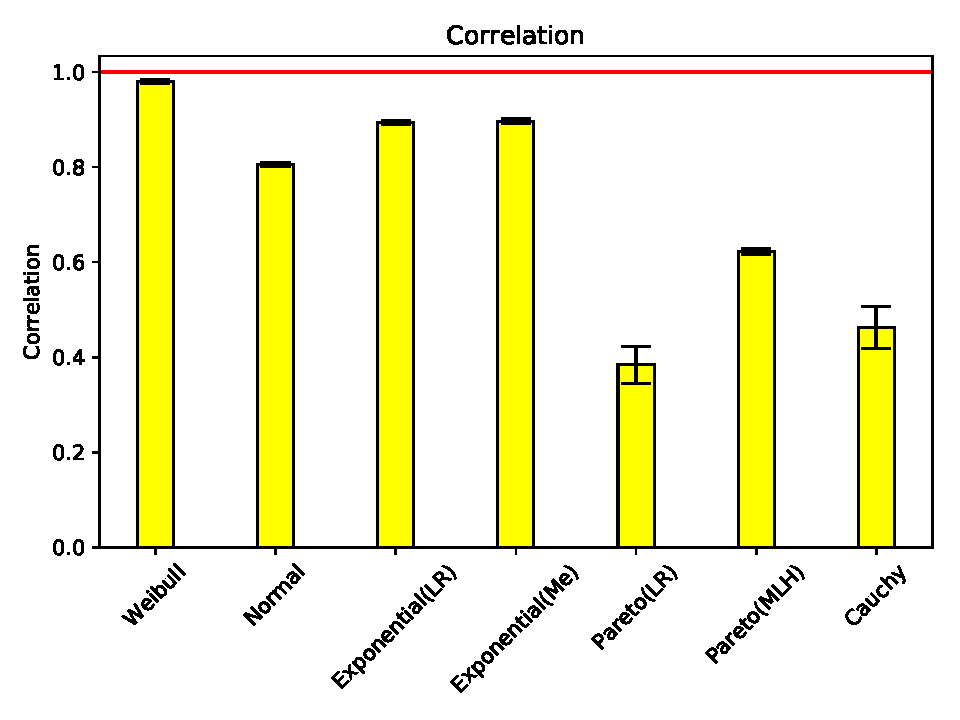
\includegraphics[width=62mm]{figures/ch4/Skype_Correlation}
        \label{correlation-skype}
    }
    \hspace{0mm}
    \subfloat[Hust Exponent]{
        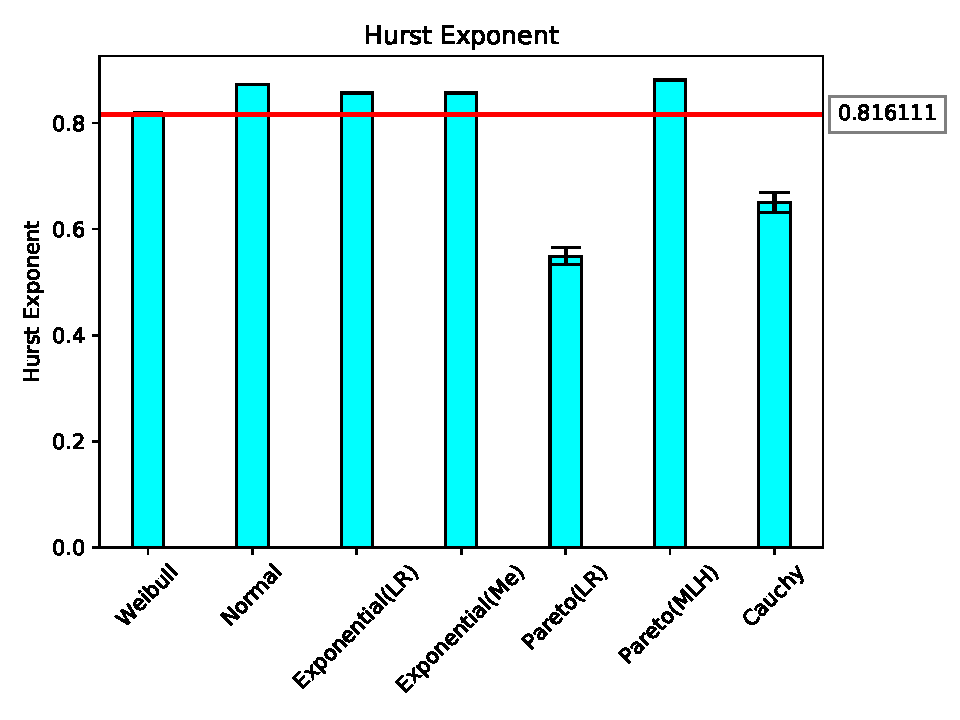
\includegraphics[width=62mm]{figures/ch4/Skype_Hurst_Exponent}
        \label{hurst-skype}
    }
    \hspace{0mm}
    \subfloat[Mean]{
        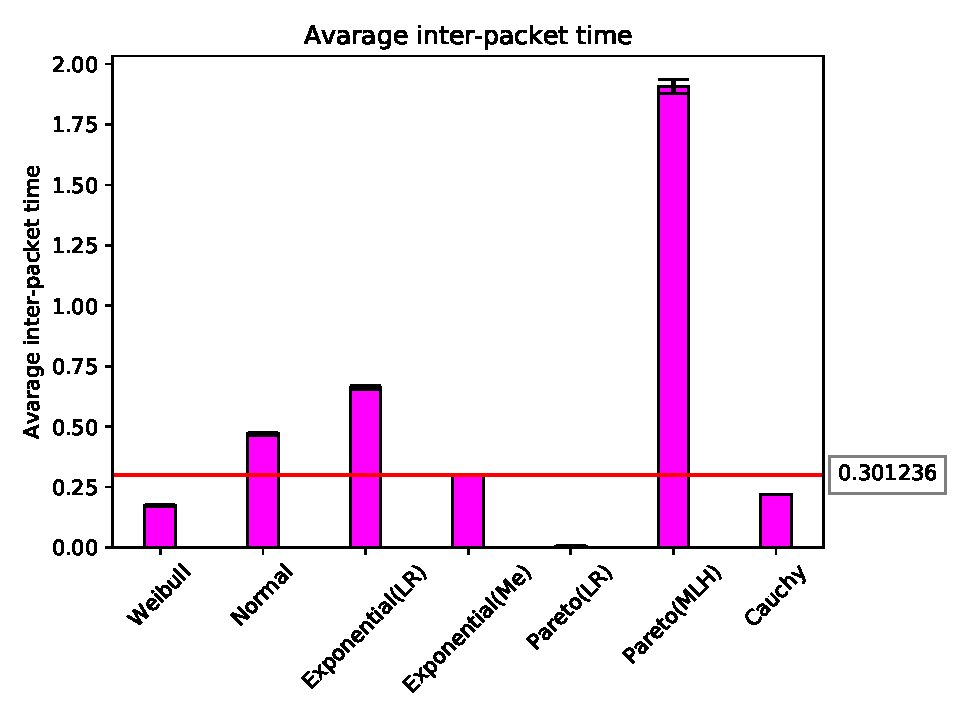
\includegraphics[width=62mm]{figures/ch4/Skype_Mean}
        \label{mean-skype}
    }
    \hspace{0mm}
    \subfloat[Standard Deviation]{
        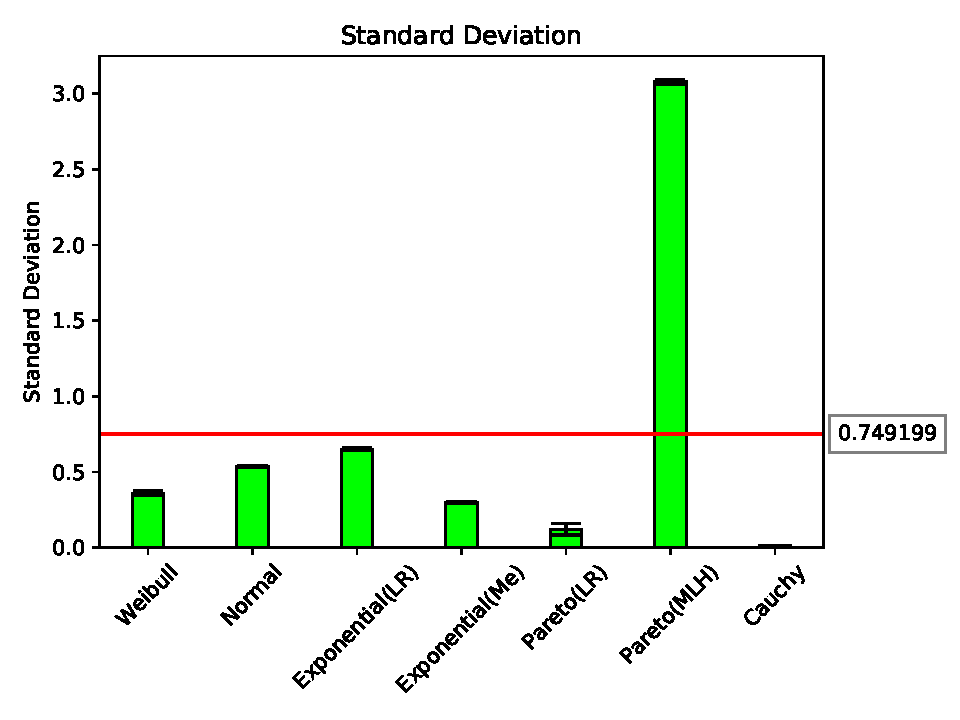
\includegraphics[width=62mm]{figures/ch4/Skype_Standard_Deviation}
        \label{std-skype}
    }
    \caption{Statistical parameters of \textit{skype-pcap} and its approximations}
    \label{fig:correlation-hurst-skype-pcap}
\end{figure}
%%%%%%%%%%%%%%%%%%%%%%%
% bigFlows -  Correlation, Hurst, Mean Standard Deviation
%%%%%%%%%%%%%%%%%%%%%%%
\begin{figure}[ht]
    \centering
    \subfloat[Correlation]{
        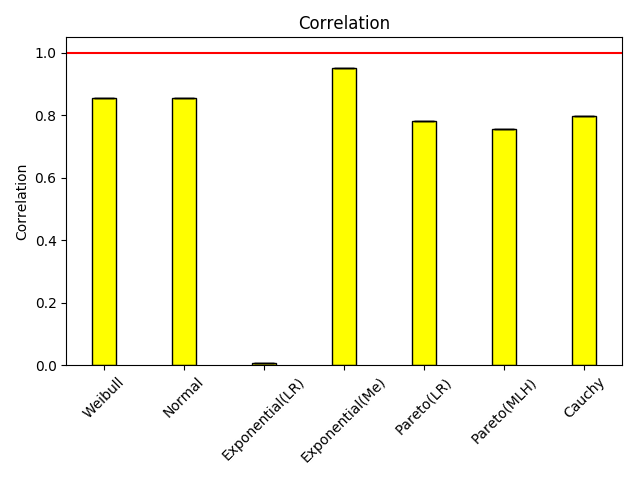
\includegraphics[width=62mm]{figures/ch4/bigFlows_Correlation}
        \label{bigFlows-correlation-skype}
    }
    \hspace{0mm}
    \subfloat[Hust Exponent]{
        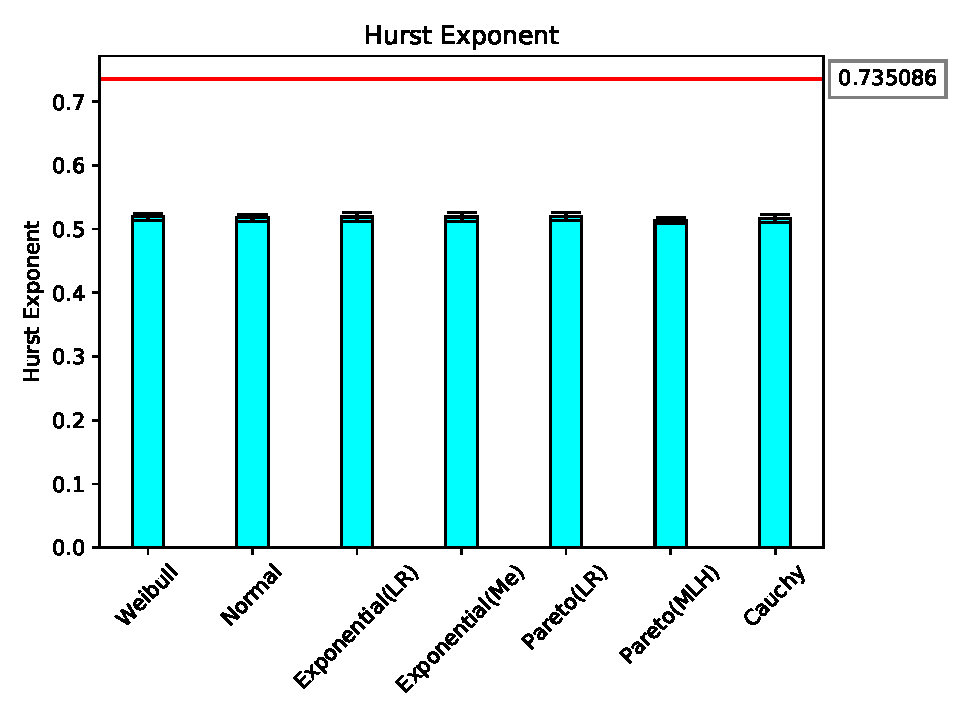
\includegraphics[width=62mm]{figures/ch4/bigFlows_Hurst_Exponent}
        \label{bigFlows-hurst-skype}
    }
    \hspace{0mm}
    \subfloat[Mean]{
        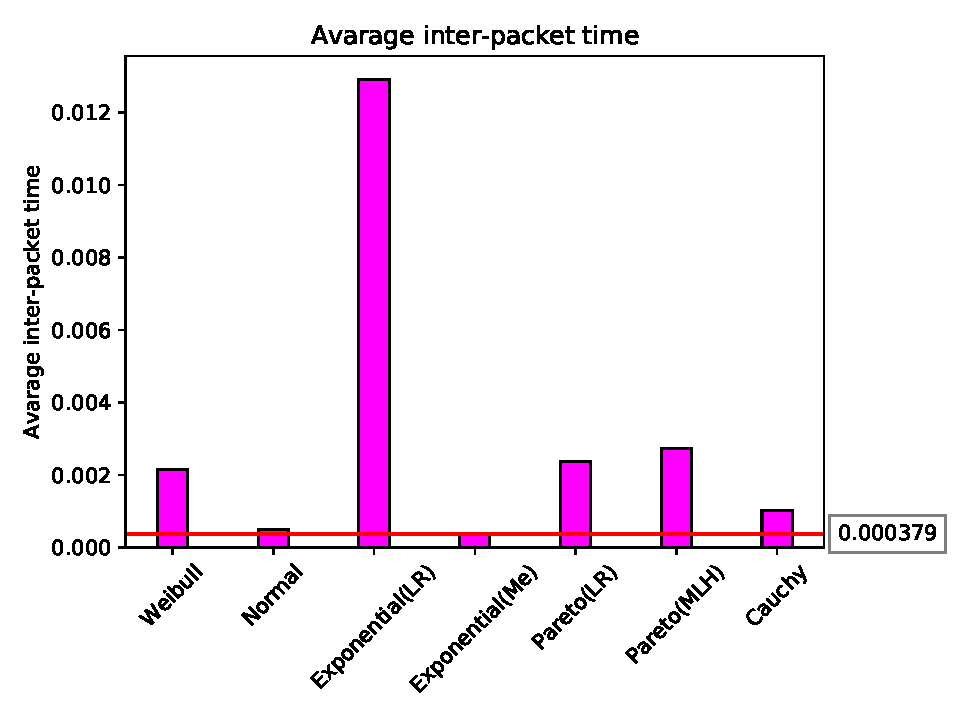
\includegraphics[width=62mm]{figures/ch4/bigFlows_Mean}
        \label{bigFlows-mean-skype}
    }
    \hspace{0mm}
    \subfloat[Standard Deviation]{
        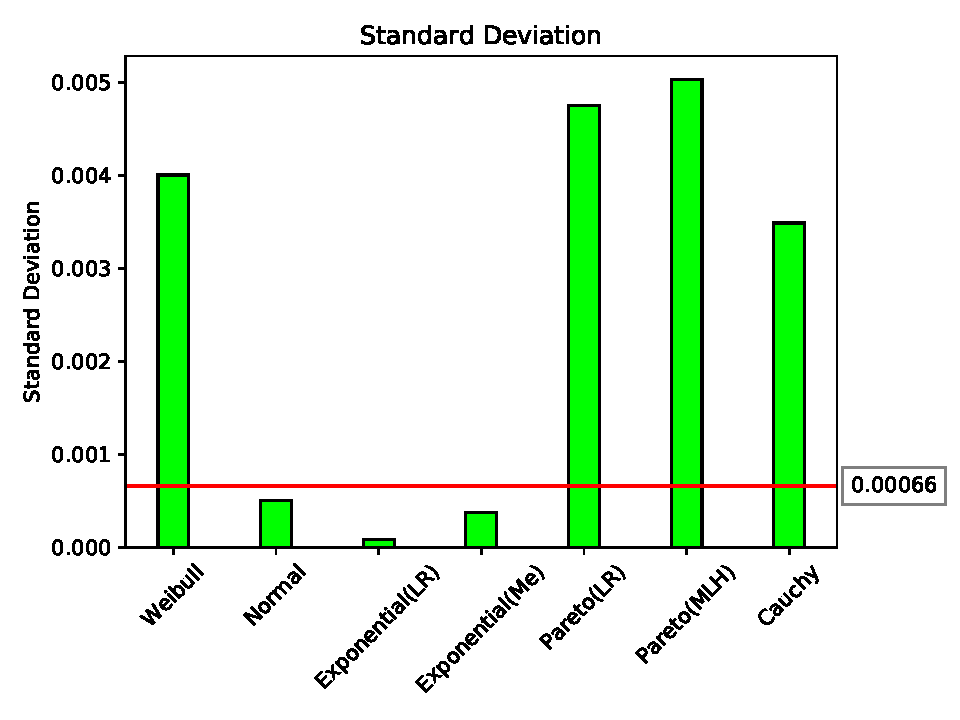
\includegraphics[width=62mm]{figures/ch4/bigFlows_Standard_Deviation}
        \label{bigFlows-std-skype}
    }
    \caption{Statistical parameters of \textit{lan-gateway-pcap} and its approximations}
    \label{fig:correlation-hurst-lan-gateway-pcap}
\end{figure}

%%%%%%%%%%%%%%%%%%%%%%%
% lanDirunal  - correlation, Hurst, Mean Standard Deviation
%%%%%%%%%%%%%%%%%%%%%%%
\begin{figure}[]
    \centering
    \subfloat[Correlation]{
        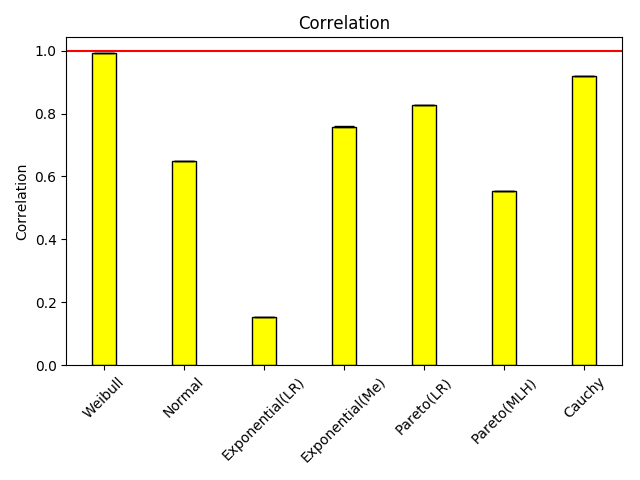
\includegraphics[width=62mm]{figures/ch4/Lan_Correlation}
        \label{Lan-correlation-skype}
    }
    \hspace{0mm}
    \subfloat[Hust Exponent]{
        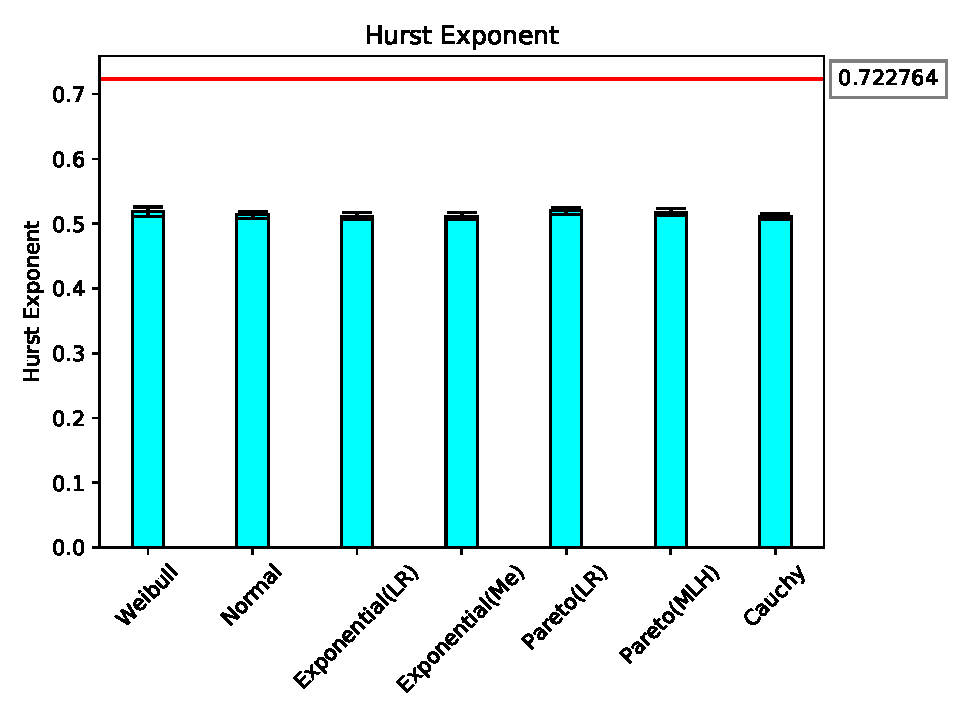
\includegraphics[width=62mm]{figures/ch4/Lan_Hurst_Exponent}
        \label{Lan-hurst-skype}
    }
    \hspace{0mm}
    \subfloat[Mean]{
        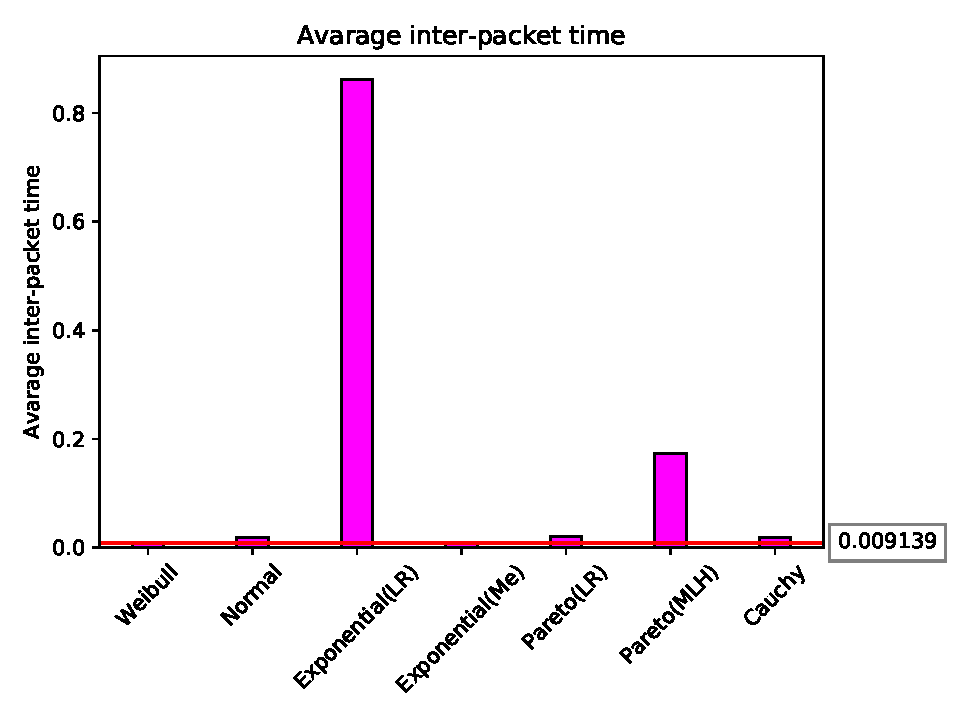
\includegraphics[width=62mm]{figures/ch4/Lan_Mean}
        \label{Lan-mean-skype}
    }
    \hspace{0mm}
    \subfloat[Standard Deviation]{
        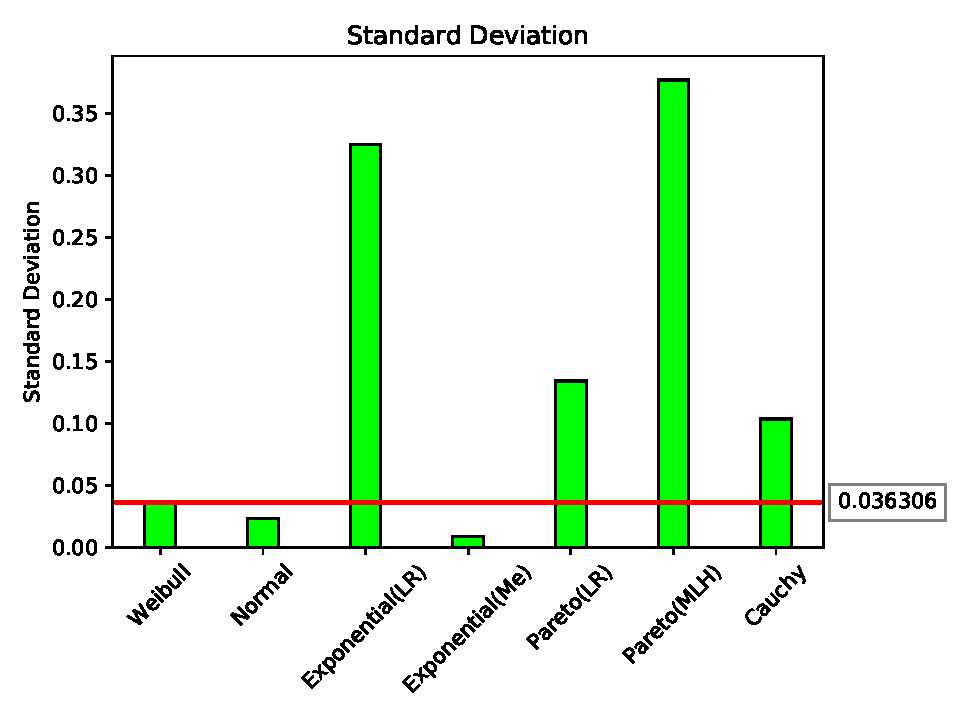
\includegraphics[width=62mm]{figures/ch4/Lan_Standard_Deviation}
        \label{Lan-std-skype}
    }
    \caption{Statistical parameters of \textit{Lan-pcap} and its approximations}
    \label{fig:correlation-hurst-Lan-pcap}
\end{figure}

%%%%%%%%%%%%%%%%%%%%%%%
% Wan - correlation, Hurst, Mean Standard Deviation
%%%%%%%%%%%%%%%%%%%%%%%
\begin{figure}[]
    \centering
    \subfloat[Correlation]{
        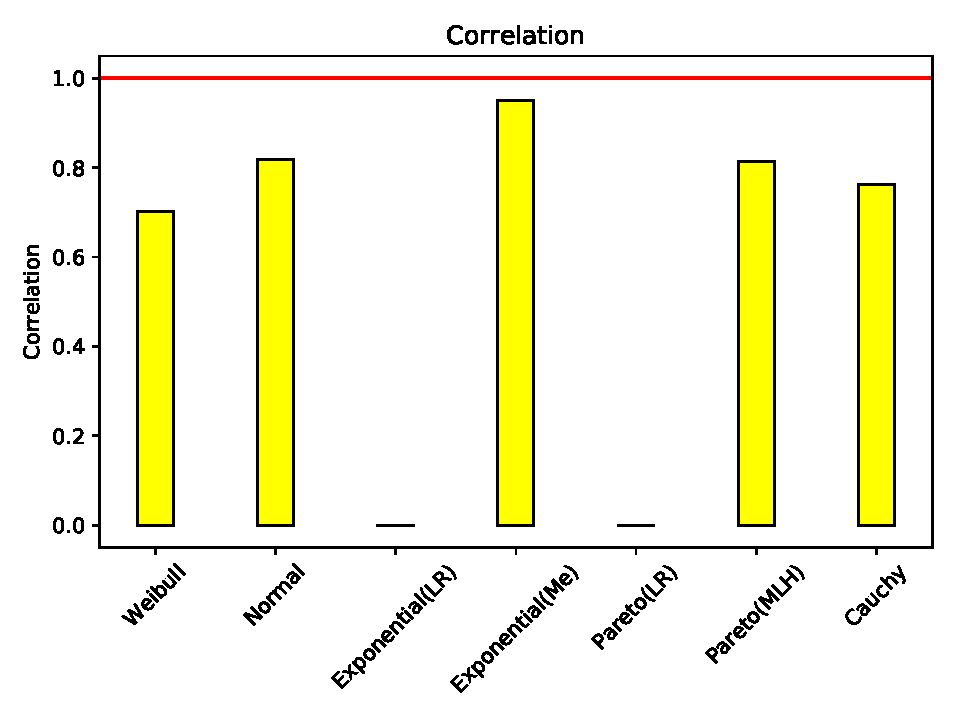
\includegraphics[width=62mm]{figures/ch4/Wan_Correlation}
        \label{Wan-correlation-skype}
    }
    \hspace{0mm}
    \subfloat[Hust Exponent]{
        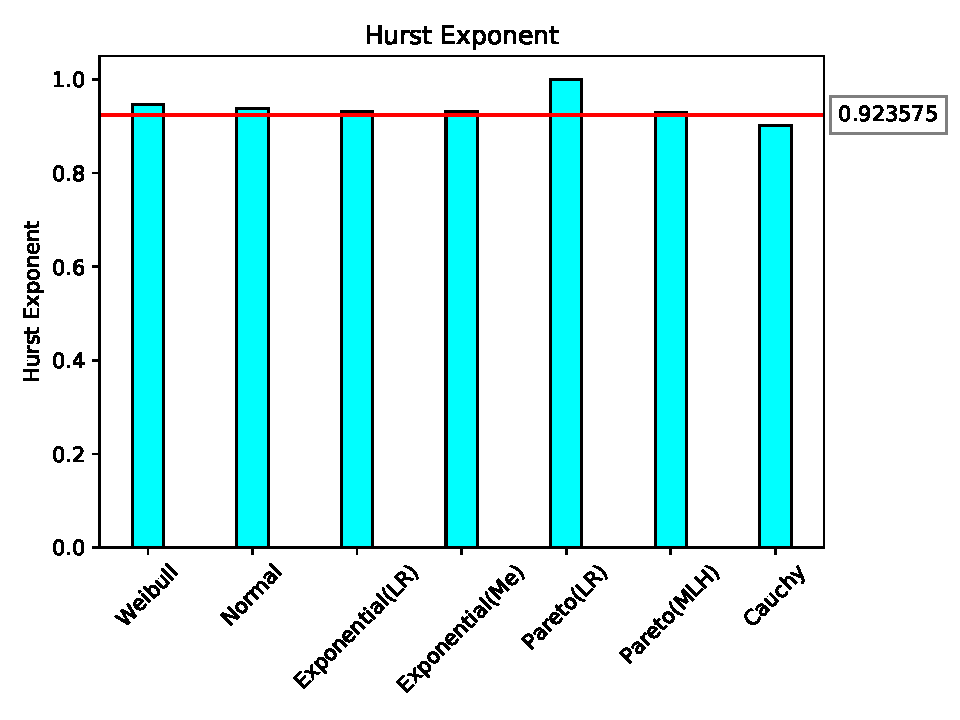
\includegraphics[width=62mm]{figures/ch4/Wan_Hurst_Exponent}
        \label{Wan-hurst-skype}
    }
    \hspace{0mm}
    \subfloat[Mean]{
        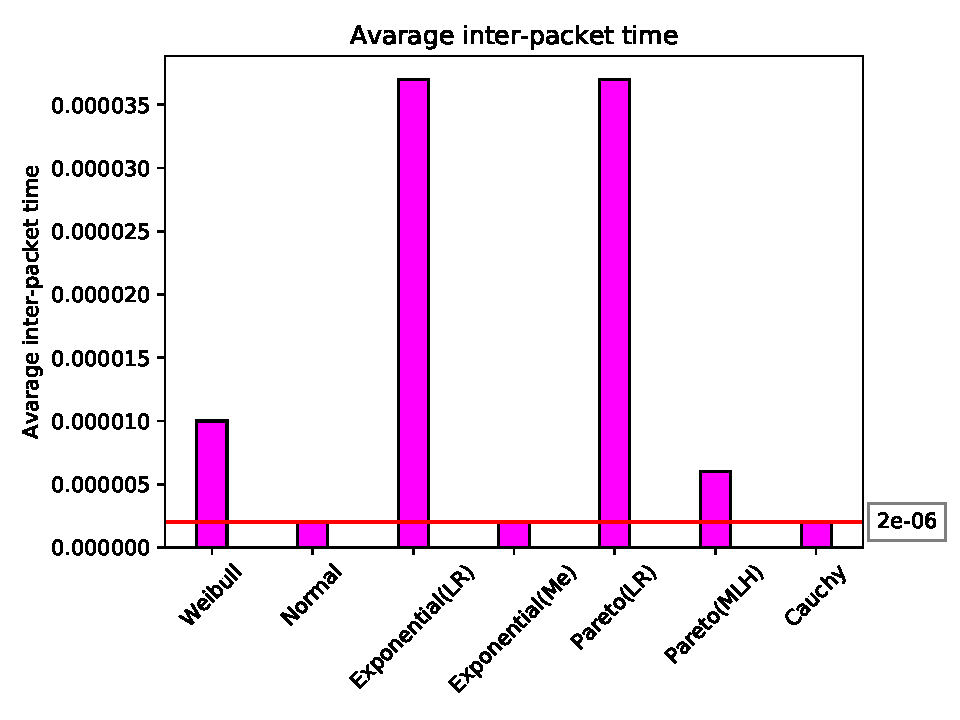
\includegraphics[width=62mm]{figures/ch4/Wan_Mean}
        \label{Wan-mean-skype}
    }
    \hspace{0mm}
    \subfloat[Standard Deviation]{
        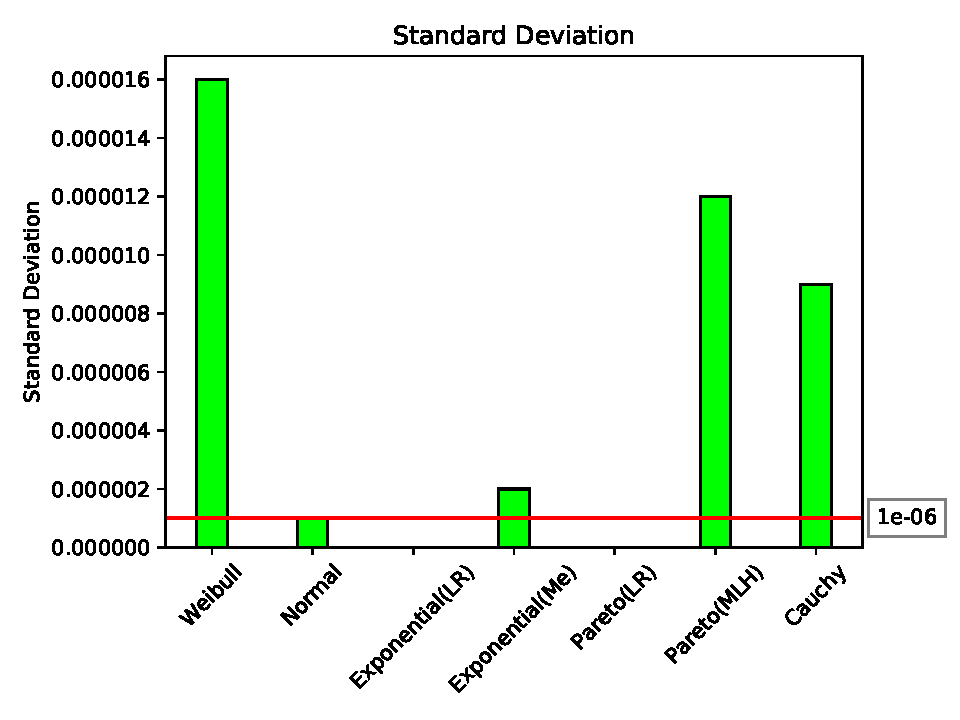
\includegraphics[width=62mm]{figures/ch4/Wan_Standard_Deviation}
        \label{Wan-std-skype}
    }
    \caption{Statistical parameters of \textit{wan-pcap} and its approximations}
    \label{fig:correlation-hurst-wan-pcap}
\end{figure}

%%%%%%%%%%%%%%%%%%%%%%%
%validation Cost function
%%%%%%%%%%%%%%%%%%%%%%%
\begin{figure}[t!]
    \centering
    \subfloat[\textit{skype-pcap}]{
        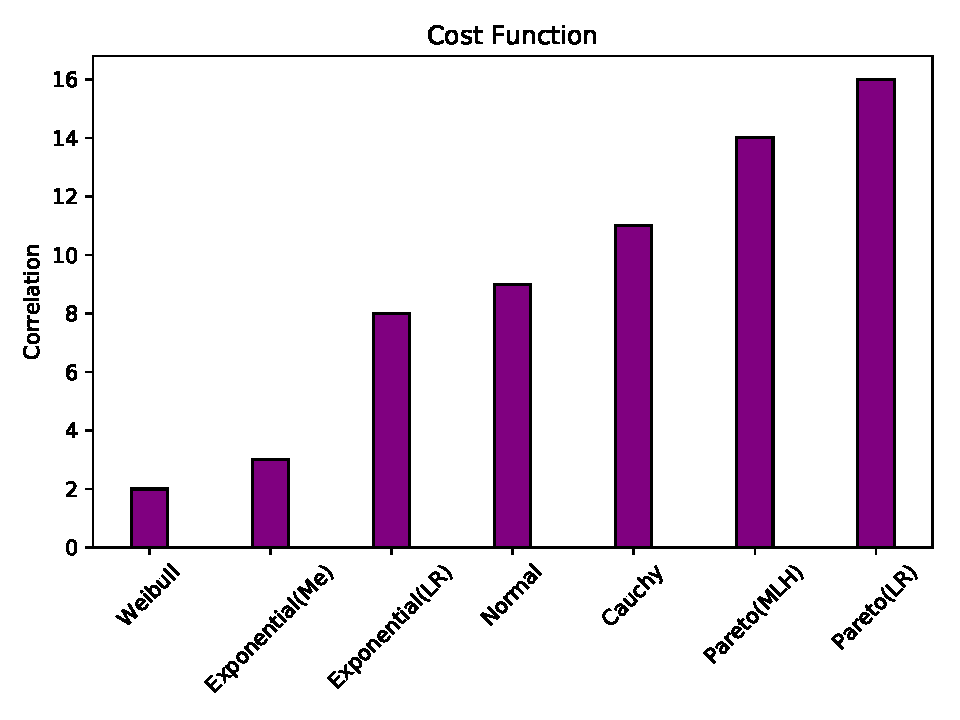
\includegraphics[width=62mm]{figures/ch4/Skype_costFunction}
        \label{cost-skype-pcap}
    }
    \hspace{0mm}
    \subfloat[\textit{lan-gateway-pcap}]{
        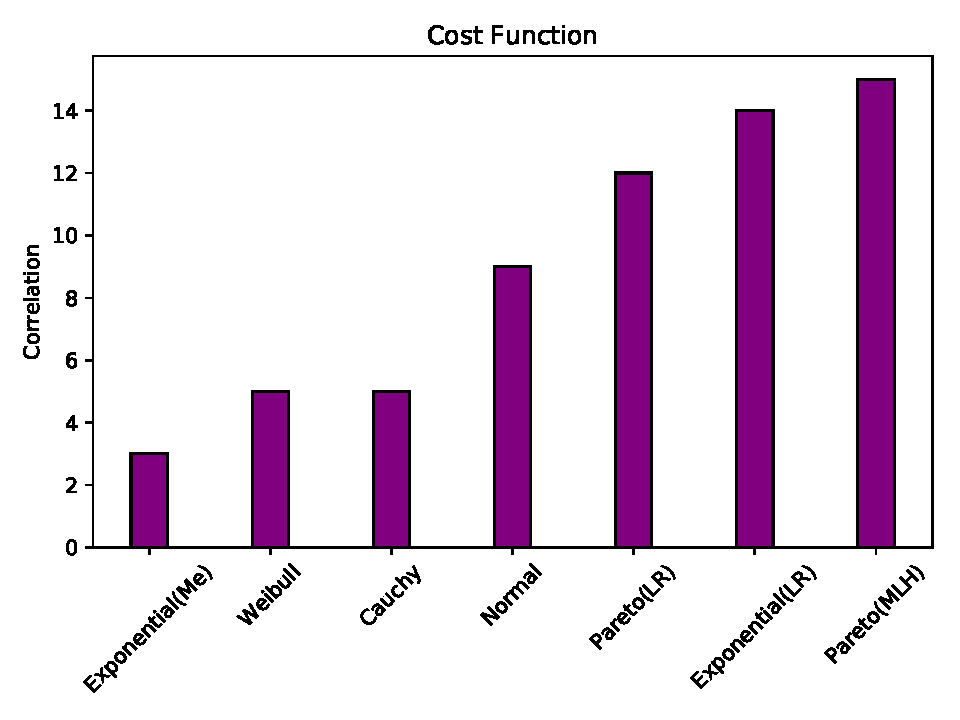
\includegraphics[width=62mm]{figures/ch4/bigFlows_costFunction}
        \label{cost-lan-gateway-pcap}
    }
    \hspace{0mm}
    \subfloat[\textit{lan-firewall-diurnal-pcap}]{
        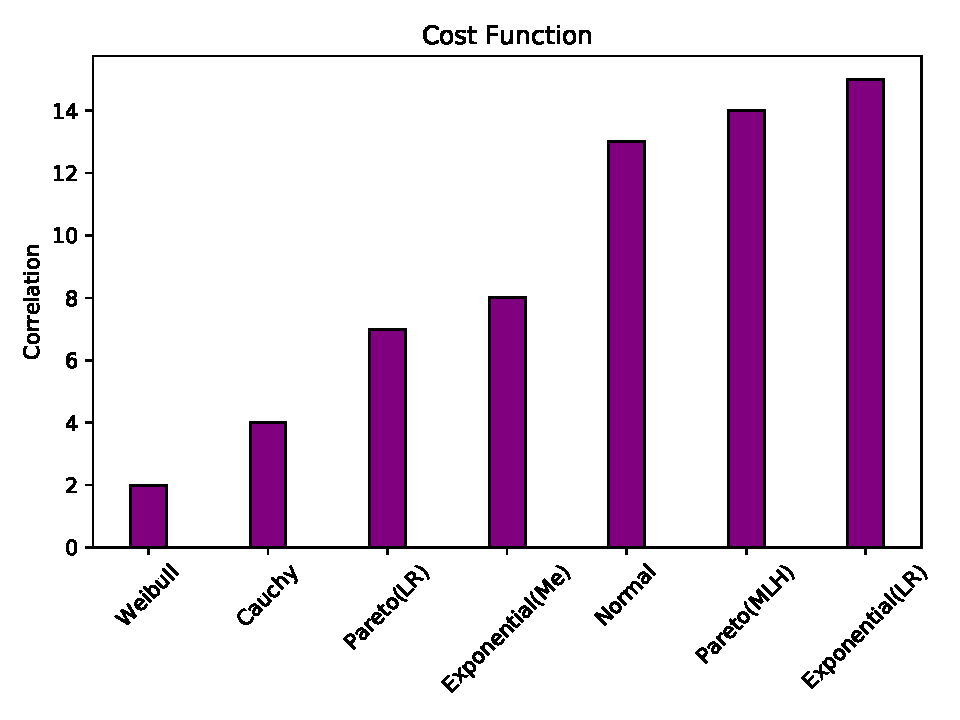
\includegraphics[width=62mm]{figures/ch4/Lan_costFunction}
        \label{cost-lan-pcap}
    }
    \hspace{0mm}
    \subfloat[\textit{wan-pcap}]{
        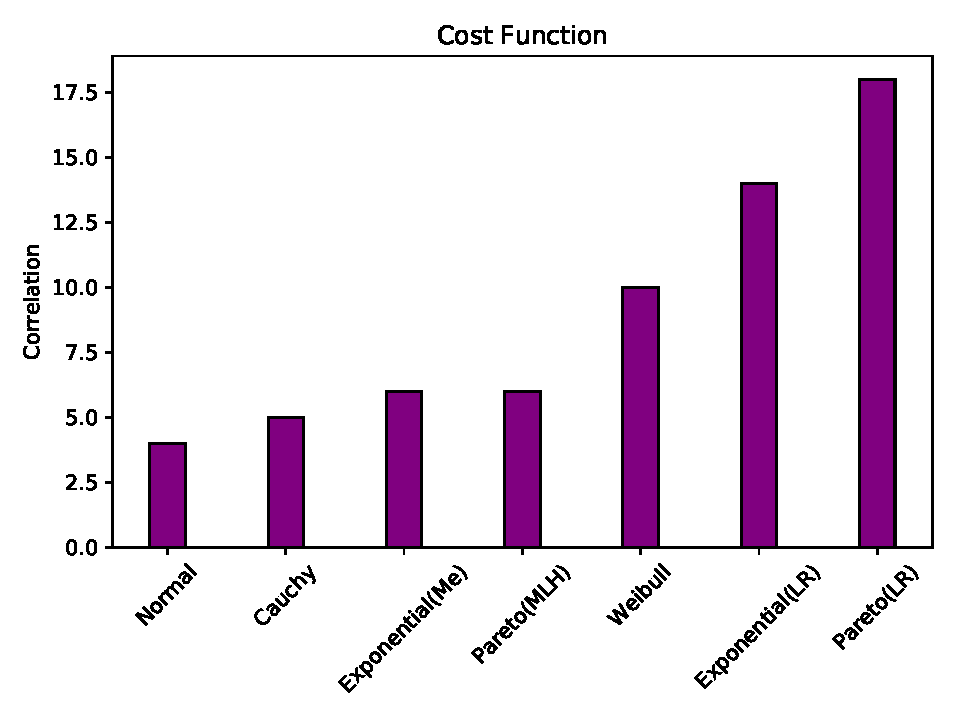
\includegraphics[width=62mm]{figures/ch4/Wan_costFunction}
        \label{cost-wan-pcap}
    }
    \caption{Cost function for each one of the datasets used in this validation process}
    \label{fig:cost-function}
\end{figure}

%%%%%%%%%%%%%%%%%%%%%%%
%validation Cost function
%%%%%%%%%%%%%%%%%%%%%%%
%\begin{figure}[t!]
%    \centering
%    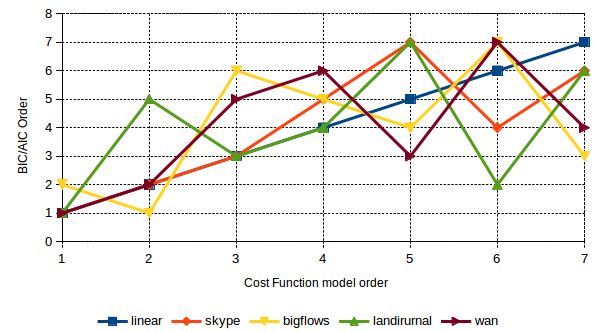
\includegraphics[width=100mm]{figures/ch4/aic-bic_vs_costFunction_order}
%    \caption{Comparison of model selection order com cost function and AIC/BIC}
%    \label{fig:cost-function_vs_aic-bic}
%\end{figure}

\begin{figure}[!ht]
	\centering
	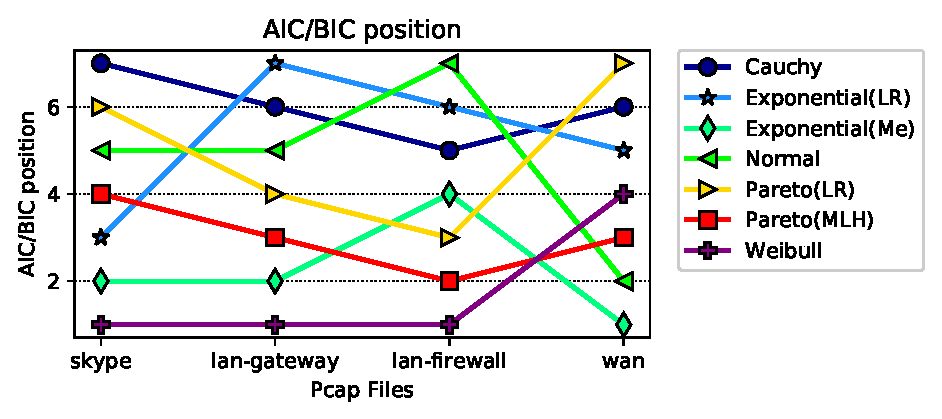
\includegraphics[scale=0.8]{figures/ch4/aic-bic-order}
	\caption{Comparision of the quality order of each model given by AIC and BIC}
	\label{fig:aic-bic-order}
\end{figure}


\begin{figure}[ht!]
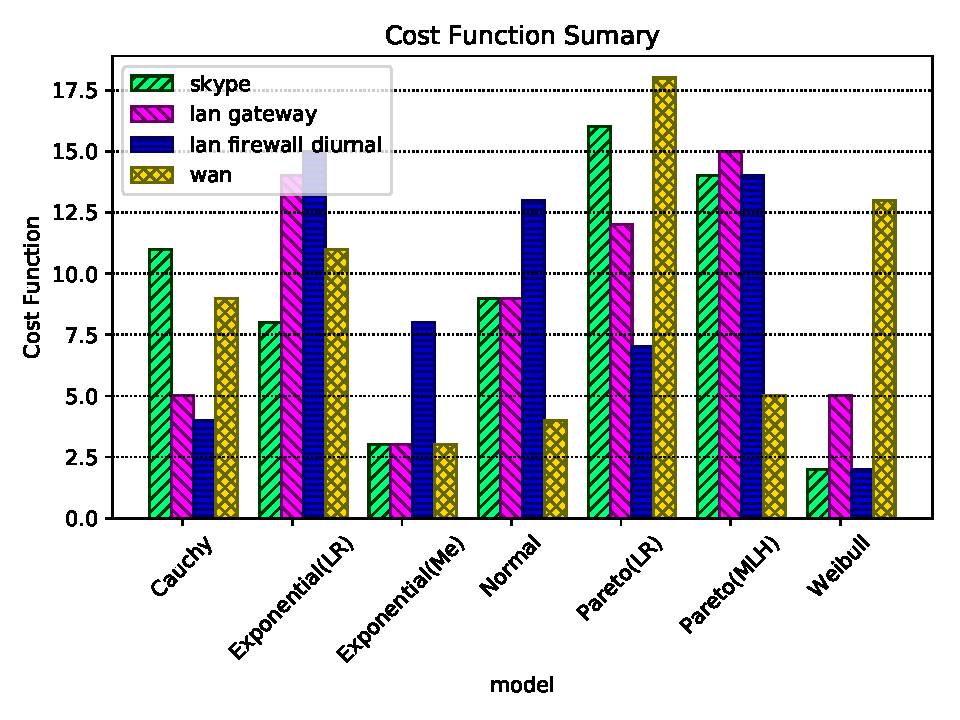
\includegraphics[scale=0.8]{figures/ch4/cost-function-summary}
\caption{Cost function for each one of the datasets used in this validation process.}
\label{fig:model-order-cost}
\end{figure}

\begin{figure}[ht!]
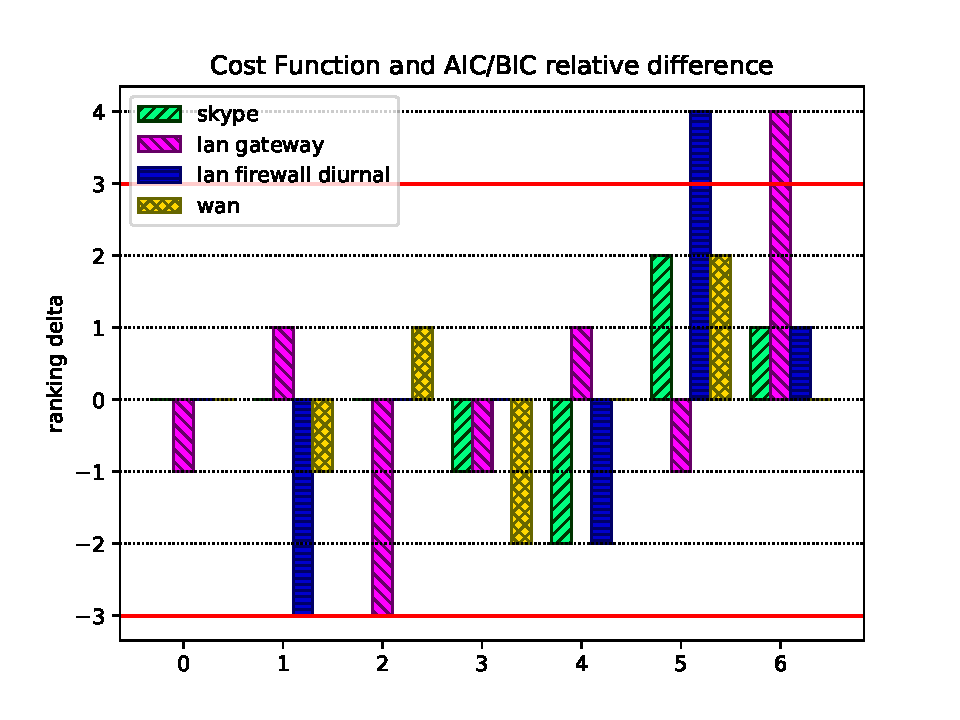
\includegraphics[scale=0.8]{figures/ch4/aicbic-costfunction-relative-diff}
\caption{Comparison of the model selection order for $BIC$/$AIC$ and the cost function $J$ for each \textit{pcap}.}
\label{fig:cost-function_vs_aic-bic}
\end{figure}



\begin{algorithm}[ht!]
    \caption{stochasticModelFitting}
    \label{alg:stochasticModelFitting}
    \begin{algorithmic}[1]
        \small        \Function{stochasticModelFitting}{$interArrivalData, criterion$}
        \State $m = interArrivalData.size$
        \State $interArrivalData = interArrivalData + MIN\_TIME$
        \If{$m < MINIMUM\_AMOUNT\_OF\_PACKETS$}
        \State $model\_list = \{constant\}$
        \Else
        \State $model\_list = \{weibull, pareto\_lr, pareto\_mlh, exponential\_me, exponential\_lr, normal,$
        \State $cauchy, constant\}$
        \EndIf
        
        \For{$model$ \textbf{in} $model\_list$}
        \State $model.fitting\_model(interArrivalData)$
        \EndFor
        \State $model\_list.sort(criterion)$
        \State \textbf{return} $model\_list$
        \EndFunction
    \end{algorithmic}
\end{algorithm}

Here in this chapter we only discuss the plots achieved obtained by the \textit{pcap} \textit{skype-pcap} for simplicity. The other plots are provided and commented on the appendix ~\ref{ap:aditional-plots}. In the figure~\ref{fig:aproximation-original-cdf} we present all estimated CDF functions along with the empirical CDF, for the trace \textit{skype-pcap}. They are on log-scale, which provide a better visualization for small time scales. In the case of the normal function, all values smaller than zero were set to zero on the plot. Is possible to see different accuracies and types of fittings on each plot. Visually, the best fit seems to be the Weibull trough linear regression. 

Analyzing the plots, and what they would mean, our Cauchy fitting would impose almost constant traffic, with the inter-packet time close to the mean. On the trace \textit{skype-pcap} the exponential plots seems not to represent well the small values of inter-packet times. This is due fact that an exponential process is good at describing values close to the average. But, it fails to represent values too small and higher. On the other hand, a self-similar process like Weibull and Pareto are better serving inter-packet times with higher dispersion. Pareto(MLH) has a slow convergence, which means this distribution may generate values of inter-packet times too large. 

Analyzing the QQplots, we can observe that in most of the distribution, the samples (original data) has a much havier-tail effect than in the estimated data. We can verify this by the by the almost blue horizontal lines formed by the x-marks. But, the Weibull distribution follows much closer the original data. Also is possible to see that the sample has a right skew compared to the estimation on Exponential(LR), Exponential(Me), Normal, and Pareto(MLH). This "right-skew" means that this estimation would not represent so well small values of time in this case. On the other hand, Pareto(LR) and Weibull would not suffer from this problem.

The results for the AIC, BIC, and parameters of all four traces are at the table~\ref{tab:prototype-results}.  The results for \textit{wan-pcap} and \textit{lan-firewall-diurnal-pcap} are on the table ~\ref{tab:prototype-results}. The differences between BIC and AIC values from a same stochastic function all cases are small compared to the difference between their values calculated between different distributions. Since we compared many different types of Ethernet traces, this result indicates that for inter-packet times, use AIC or BIC as decision criteria should not influence the results from most of the cases. 

On our previsions, Weibull and Pareto(MLH and LR) are the best options. We expected that since both are heavy-tailed functions. But Cauchy on most of the tests, even being a heavy-tailed distribution, seems to no present a proper fitting. The quick divergence of the tangent function is the cause for this lousy fitting.

Analyzing the quality of AIC and BIC as criteria of choose on \textit{skype-pcap}, based on the results form figure ~\ref{fig:correlation-hurst-skype-pcap} we see that concerning Correlation and Self-similarity it picked the right model: Weibull. Also regarding average packet rate and dispersion, it is still one of the best choices (along with Exponential(Me), Pareto(LR) and Cauchy). The third and the fourth choices (Pareto(LR)) and Exponential(LR) also are good options in most of these metrics. But, Pareto(MLH) is presented as the second best choice, and it had poor results in comparison to the others, especially on mean, correlation and dispersion. 

All these results are abstracted by the cost function $J$. As we can see, on all pcaps, the best function selected by BIC and AIC(table~\ref{tab:prototype-results}) also had the small cost(figure~\ref{fig:cost-function}). 

Another important observation is the fact that exponential function was able to provide the best fitting for the \textit{wan-pcap}. The reasons for this behavior are both results of a much great traffic with no long-range gaps, and the precision of the measurement.


Since there is a lot of information on table~\ref{tab:prototype-results} and on the figure~\ref{fig:cost-function}, we capture just the order of choise form each \textit{pcap} plotted on the figure~\ref{fig:cost-function_vs_aic-bic}. We can see that expecially on the best fittings, the results were closer. Just for the \textit{lan-gateway-pcap} the results from the best and second best models were flipped. On all the other cases, the choises were the same. For the worsts models, the results tend to differ more, and loose correlation. It is not a bad thing, since they were not good choices after all. 



\subsection{Conclusion}


We can conclude that using AIC or BIC as criteria for choosing good models for inter-packet times is a good choice.

Except by the Pareto function modeled using the Maximum likelihood method, have comparative results between the simulations and the AIC/BIC goes. The best fittings according to the AIC/BIC usually returned very accurate models, with a small error between the mean and fractal level, and correlation close to one. The models selected as the worsts traditionally yielded poor results.

It is important to notice that in some cases, some stochastic functions may perform poorly, and in other provide an accurate fitting, what justify the application of the criteria in all new experiments. For example, Weibull usually plays pretty well, but in some cases, perform poorly, or may even diverge. 

We do not rely on only one type of parameterization. This approach turns our methodology more robust, since a linear regression may diverge. But always there will be a peaceable model, since our estimations for Normal, Exponential (Me) and Pareto (MLH) cannot. Models which the linear regression diverges will have very high and positive BIC/AIC estimations, and will not stand as primary options.


\section{ON/OFF Periods and Application classification}

    
\begin{algorithm}[ht!]
    \caption{calcOnOff}
    \label{alg:calcOnOff}
    \begin{algorithmic}[1]
        \small
        \Function{calcOnOff}{$arrivalTime, deltaTime, cutTime, minOnTime$}%\Comment{Where A - array, p - left, q - middle, r - right}
        \State $m = deltaTime.length() - 1$
        \State $j = 0$
        \State $lastOff = 0$
        \State $pktCounterSum = 0$
        \State $fileSizeSum = 0$
        \For{$i = 0:m$}
        \State $pktCounterSum = pktCounterSum + 1$
        \State $fileSizeSum = fileSizeSum + psSizeList[i, 1]$
        \If{$deltaTime[i] > cutTime$} 
        \If{$i == 1$} \Comment{if the first is session-off time}
        \State $j++$
        \State $onTimes.push(minOnTime)$
        \State $offTimes.push(deltaTime[i])$
        \State $pktCounter.push(pktCounterSum)$
        \State $fileSize.push(fileSizeSum)$
        \State $pktCounterSum = 0$
        \State $fileSizeSum = 0$
        \Else \Comment{base case} 
        \State $pktCounter.push(pktCounterSum)$
        \State $fileSize.push(fileSizeSum)$
        \State $pktCounterSum = 0$
        \State $fileSizeSum = 0$
        \If{$j == 0$}
        \State $onTimes.push(arrivalTime[i - 1])$
        \State $offTimes.push(deltaTime[i])$
        \Else \Comment{others on times} 
        \State  $onTimes.push(max(deltaTime[i-1] - deltaTime[lastOff], minOnTime))$ 
        \State  $offTimes.push(deltaTime[i])$
        \EndIf
        \State $lastOff = i$
        \EndIf 
        \EndIf       
        \EndFor
        \State $pktCounterSum = pktCounterSum + 1$
        \State $fileSizeSum = fileSizeSum + psSizeList[m]$
        \If{$lastOff == m - 1$} \Comment{ if last is session-off }
        \State $onTimes.push(minOnTime)$ % on time
        \Else \Comment{ base last case}
        \If{$lastOff \neq 0$}
        \State $onTimes.push(arrivalTime[m] - arrivalTime[lastOff])$ 
        \Else 
        \State $onTimes.push(arrivalTime[m])$ \Comment{there was just on time}
        \EndIf
        \EndIf
        \State $pktCounter.push(pktCounterSum)$
        \State $fileSize.push(fileSizeSum)$
        \State \textbf{return} $onTimes, offTimes, pktCounter, fileSize$
        \EndFunction
    \end{algorithmic}
\end{algorithm}
    
\begin{table}[ht!]
    \centering
    \caption{Application match table}
    \label{tab:application-protocols}
    \begin{tabular}{lll}
        \hline
        Application Protocol & Transport Protocols & Transport Ports \\ \hline
        HTTPS               & TCP                & 443             \\
        FTP                 & TCP                & 20, 21          \\
        HTTP                & TCP                & 80              \\
        BGP                 & TCP                & 179             \\
        DHCP                & UDP                & 67, 68          \\
        SNMP                & UDP, TCP           & 161             \\
        DNS                 & UDP, TCP           & 53              \\
        SSH                 & UDP, TCP           & 22              \\
        Telnet              & UDP, TCP           & 23              \\
        TACACS              & UDP, TCP           & 49              \\ \hline
    \end{tabular}
\end{table}




In this section, we briefly show another method used by the \textit{TraceAnalyzer} component. The first to calculate the session ON and OFF times. The second classify applications based on its transport protocol and ports. In the table ~\ref{tab:methods} we summarize the stack of models used to create the Compact Trace Descriptor (CTD file). 



We developed an algorithm to calculate the times between the ON and OFF times of the \textit{files}, and the number of packets and bytes as well. It uses a list of packet arrival times(relative to the first), the time between packets and packet sizes. It defines a minimum time of ON acceptable. These times are used for two reasons:

\begin{itemize}
\item In case of a \textit{file} of just one packet, it will not produce an ON-time of zero
\item It avoids a \textit{file} On time too small, which may be less than acceptable for packet generator tools.
\end{itemize}

As explained in the previous chapter, a \textit{file} is defined by a large OFF time, we call $cutTime$. If an inter-packet $deltaTime$ time is larger than the $cutTime$ it defines an OFF time, and the ON time is calculated base on the last OFF time recorded. 
If the first $deltaTime$ defines an OFF time, or if it is the first ON time, its calculation is treated separately. In the last ON time, it is not defined by an OFF time, so we deal with it after the loop. It keeps counters to calc the number of bytes and packets within every defined ON time. It returns four vectors: $onTimes$, $offTimes$, $pktCounter$ and $fileSize$. Letting $n$ be the size of $onTimes$,  $offTimes$ has a size $n - 1$. The algorithm is presented in the Alforithm~\ref{alg:calcOnOff}.



We also developed a simple test to guess the application protocol, based on the port numbers and the transport protocol used by each flow. We currently are classifying the application protocols presented in the table ~\ref{tab:application-protocols}. If a flow matches the port number, and the transport protocol, it is classified as belonging to an application protocol.

\section{Conclusions}

In this section, we went on details on some methodologies mentioned in the chapter ~\ref{ch:architecture}. Here we avoid implementation and architecture concepts, and just discussed the methods. In this first section, we focused our research on develope a consistent method for automatic selection of stochastic functions for inter-packet times. Since we could not find any other methodology in the literature, we developt our own and tested if it is worth or not. The results showed our method satisfactory and had presented a reasonable prediction rate on the best functions. We now can ensure that it is a safe method and that AIC and BIC are good criterions for this sort of data.  We abstracted this method in the algorithm ~\ref{alg:stochasticModelFitting}. In the second section, we also present the methods used to estimate packet trains periods (algorithm ~\ref{alg:calcOnOff}) and make the application classification (table ~\ref{tab:application-protocols}). In the table ~\ref{tab:methods}, the usage of each method is summarized. 

\begin{table}[ht!]
    \centering
    \caption{Methods used by each layer.}
    \label{tab:methods}
    \begin{tabular}{cc}
        \hline
        Layer                               & Method                                 \\ \hline
        Link Layer                          & \multirow{3}{*}{Packets header's data} \\
        Network Layer                       &                                        \\
        Transport Layer                     &                                        \\
        Application Layer                   & Application Match Table                \\
        \multirow{2}{*}{Inter Packet Times} & Algorithm: $calcOnOff$                 \\
        & Algorithm: $stochasticModelFitting$    \\
        Packet Sizes                        & Algorithm: $stochasticModelFitting$    \\ \hline
    \end{tabular}
\end{table}

%\section{Implementation Details}

%\subsection{Modeling Process}

%\subsection{Matlab prototyping and C++ Implementation}

%\subsection{Software Engineering process and Lessons Learned}

%\section{Conclusion}

%We can conclude by this evaluation, that our chosen methodology for selecting stochastic models for inter-packet data is appropriated. The first thing to observe is that, for a high 

%First, we do not rely on only one type of parametrization. This turns our methodology more robust, since a linear regression may diverge. But always there will be a packable model, since our estimations for Normal, Exponential(Me) and Pareto(MLH) cannot. Models wich the linear regression diverge, will not have god BIC/AIC estimations, and will not be picked. 

% https://en.wikipedia.org/wiki/Gamma_process
%Intordução
%- Como previamente discutido, há uma farta bibliografia dedicada ao estudo da natureza do trafego de internet. Em especial, relacionada a modelos que possam expressar a natureza do tempos entre pacotes. 
%- Como discutido anteriormente, Sabemos pela literatura que o trafego de internet possui uma caracteristica fractal. Processos tipicos de Poisson (expresso em sua forma contínua por uma funções estocastica esponencial)  não são capazes de representar de maneira realistica o trafego. Para tal, podem ser utilizados processos estocasticos heavy-tailed.
%- Porém não são numerosos os trabalhos que tratam da parametrização desses processos. Qual o melhor tipo de parametirzação é uma questão difícil de ser respondida, por diversas. Primeiramente, utilizar funções heavy-tailed pode ser uma metodologia mais eficaz para se garantir a self-similarity do trafego. Porém não necessáriamente outras importantes características do trafego serão mantidas, como por exemplo: média de pacotes por segundo, disperssão e correlação entre o trafego real e o trafego sintético gerado por esse processo. Não há a prncípio uma carantia que a escolha baseada em self-similatrity também irá garantir que essas outras características se mantanham. O ideal é que  encontremos um método que possa garantir um bom resultado na maioria, se não em todas essas características.
%- Além disso, há diversos métodos disponíveis para se estimar parâmertos de uma função estocastica. Para citar alguns exemplos:
%* Em alguamas funções como a normal e a exponencial os parâmetros podem ser estimados diratemente através do calculo da média e da variância dos dados.
%* Em funções que é possivel realizar a linearização, os parametros podem ser estimados por meio de regressão linear
%* Outro método frequentemente usado é o do maximum likelihood
%Porém, prever comportamento que cada funções estocástica terá com cada um desses estimadores, não é trivial. Por exemplo.  Por exemplo:
%* Dependendo dos dados originais, a estimativa pode ser muito pobre, e posuir uma baixa correlação com os dados originais. 
%* Os estimadores possuirão algum "bias", desviando apresentando um desvio para cima ou para baixo no valor esperado. Ou isso pode não ocorrer.
%- O objetivo desse capítulo é somente avaliar a qualidade de nosso modelo para estimativa de parâmetros estocasticos para estimadores de inter packet times. iremos utilizar o nosso procedimento em diferentes datasets, e avaliar a qualidade dos resultados obtidos.

\begin{comment}

%%%%%%%%%%%%%%

%To evaluate the quality of the generated data, we use four criteria: 

%As we can see in the figure~\ref{correlation-skype-pcap}, Weibull has a correlation close to one correlation (0.969). The follow values of next values of correlation are: Pareto(LR)(0.810), Normal (0.701), Exponential(LR) (0.697), Pareto(MLH) (0.556), Cauchy (0.470), and Exponential(Me) (0.294).

%The next criterion is The Hurst exponent. First, we can observe that all fittings have resulted in a  self-similar process since all values were between 0.5 and 1. Again, the AIC prediction was confirmed, since the Weibull fitting is the one with the closest fractal level from the original trace, around 0.80 and 0.85.

Revisão da literatura
* O trabalho do sourcesonoff realisa uma análise extensiva de uma modelagem apropriada entre bursts de trafego. No trabalho, algumas funções estocasticas são analizadas, e é recomendado o uso sa Weibull. Nesse trabalho é utilizado o calculo do prâmetro BIC como estimador da melhor função estocastica


Metodologia e validação
- por questões referentes a teoria da iinformação, optamos por utilizar o parametro AIC como nosso estimador oficial de melhor função estocastica. 
- Porém, também calculamos o BIC, e verificamos ue via de regra a diferença dos dois valores é bem baixa. Em geral, para datasets maiores, a diferença entre o BIC e AIC de uma mesma função tende a ser consideravelmente menor do que se comparado ao de outra funçao, como veremos a seguir
- A metodologia escolhida é a seguinte: realizamos a estimativa de parametors de diversas funções estocasticas para um mesmo dataset. Calcularemos o valor do AIC, e baseado nele, iremos estimar, em ordem crescente qual a melhor função estocástica. 
- fazer uma figura com cores, mostrando segundo o estimador a ordem das funções, e compara-las com  a ordem estimada por meio dos 4 outros parâmetros.
 - Utiizar correlação, media, variancia, e hurst.
- A vantagem do AIC é que tendo a disposição o datset original, ele é um metodo completamente analítico, não dependendo da geração de numeros aleatórios (como por exemplo no cauculo da correação). Nesse caso, evita que o gerador escolhido possua algum bias na geração dos dados, e comprometa o resultado do estimaor. Além disso, é um procedimento computacionalmente mais barato, pois é puramente analitico

Resultados
- Neste capítulo apresentaremos a análise de somente  2 datasets: da captura de skype e da captura big-flows. No apendice haverão outras análises, que incluem:
* uma análise de inter packets times de uma captura diurnal
* inter-packets times de um single flow do caida
* inter-burst timesconsiderando apenas inter-packet times maiores do que 1 segundo.
* inter pacekt time de 1 segundo do trace do caida.
- o porposito desse modelo é avaliar a qualidade do modelo de seleção, se ele é uma boa ou mpa escolha, já que não há muitso trabalhos relacionados na literatura.
- como o trafego de internet é fractal, caso essa metodologia represente uma boa escolha para os datsets analisados, ele também tende a ser uma boa escolha para datasets de diferentes intervalos de inter-packet times (maiores e menores). Uma análise mais precisa é feita no apendice a respeito dessa questão.






Conclusões







%In this chapter we will go deep into details on how our tool makes the data modeling, focusing on inter-packet times. We will present curves obtained by our Matlab prototype that shows in detail how each step works. After explaining this process, we will display an evaluation method of our results, using \textit{QQplots}. After this, we give some details of how we convert code from Matlab to C++ and its benefits on time execution. All code used in this section is available on our GitHub page, in the directory \texttt{Prototypes}. 

%We also define here the datasets we are going to use in the rest of this text. We will use two datasets, and for reproduction purposes, one is publicly available. The first is a CAIDA\footnote{http://www.caida.org/home/}{http://www.caida.org/home/}, and can be found at  \href{https://data.caida.org/datasets/passive-2016/equinix-chicago/20160121-130000.UTC}{https://data.caida.org/datasets/passive-2016/equinix-chicago/20160121-130000.UTC}. Access to this file need login, so you will have to create an account and wait for approval first. The pcap's file name is \texttt{equinix-chicago.dirA.20160121-130500.UTC.anon.pcap.gz}. The second we capture in our laboratory LAN, through a period of 24 hours. Along with other tests, We intend to verify diurnal behavior on it. 


%%%%%%%%%%%%%%%%%%%%%%%%%%%%%%%%%%%%%%%%%%%%%%%%%%%%%%%%%%%%%%%%%%%%%%%%%%%%%%%%


%After we implement this model, we were able to get different approximations for the stochastic functions. To evaluate how well the method can fit inter-packet times, we first test it against a whole set of inter-packet times. Figures (...) represents the CDF fitting for the function for the \textit{skype-pcap}. In the appendix ~\ref{ap:mathematical-modeling}, we also present the fitting achieved for whole set of inter-packet times, and for a single selected flow of \textit{caida-pcap} and\textit{lan-firewall-diurnal-pcap} \textit{pcaps} . We can see that the Weibull approximation fits better than any exponential approximation. But, we define an automatic way to estimate the best fitting. We  use the AIC (Akaike information criterion), which is given by:

%\begin{equation}
%AIC = 2k - 2\ln{(L)} 
%\end{equation} 

%where $k$ is the number os estimated parameters for the stochastic function, and $L$ is the value of the likelihood function. We explain it in details in the appendix A. The smaller is the AIC value, the best is the function fitting. An alternative for the AIC is the BIC value, which follows the same rule. This equation defines BIC:

%\begin{equation}
%BIC = k\ln{(n)} - 2\ln{(L)}
%\end{equation}

%where n is the number of elements of the sample dataset. We present at table ~\ref{tab:bic-aic} the values found by each estimator, for the \textit{skype-pcap}.

%As we can see, both BIC and AIC agree on each element, which one is the best and the worst. In this case, the best is the Weibull, and the worst is the Cauchy. The exponential models, which are the continuous version of a classical Poisson process, is worse than Weibull and both Pareto estimation.

%But, to verify if our estimation is reasonable, we need to see what sort of data these stochastic processes can generate, and how close the stochastic properties of the synthetic dataset is from the original. In this way, we will be able to verify its actual quality in an unbiased way.



% The Pearson correlation is +1 in the case of a perfect direct (increasing) linear relationship (correlation), −1 in the case of an ideal decreasing (inverse) linear relationship



%\textcolor{red}{TODO:Fazer uma breve avaliação das parametrizações obtidas com os dois traces utilizando QQplots, e comentar os resultados }


%\section{C codification}

%\textcolor{red}{TODO: Explicar detalhes da codificação em C, como bibliotecas utilizadas, a utilização de valores minimos para evitar o calculo de $\log{0}$, e a opção de executar testes de regressão, compilando com a opção regression-tests ou outra que eu criar na hora.}
\end{comment}
